\chapter{Deformation -- M-Processes}
\section{Theory}
%\GeoSys  (\gversion) can analyze 2D and 3D deformation
%problems of porous and fractured media. For 2D problems, we restrict the analysis under the
%assumption of plane strain.  Triangle and quadrilateral element
%types are available for 2D simulation. While, 3D simulations can
% use tetrahedron, hexahedron, prismatic elements.

Pure deformations in any media  can be described by the momentum
balance equation in the terms of stress as
\begin{equation}
\nabla \cdot \Stress + \dens\grv = 0
\label{eq:momb}
\end{equation}
where $\Stress$ is stress tensor, $\dens$ is the solid density. In the present implementation, the traditional sign
convention for stress and fluid pressure is used. Displacement $\Disp$ is the primary variable to be solved by
substituting the constitutive law for stress-strain behavior
\begin{equation}
\begin{array}{l}
 \Stress = \CT\, \StrainT\\
  \StrainT = \dfrac{1}{2}(\nabla \Disp+(\nabla \Disp)^{\mathrm T})
 \end{array}
 \label{eq:strstr}
\end{equation}
with $\CT$, a forth order material tensor and $\StrainT$, the
strain. Superscript $\mathrm T$ means the transpose of matrix. The
deformation problem can be considered as a boundary value problem
with boundary conditions given by
\begin{equation}
\Stress : \nrl = \bm t
\quad \mbox{or} \quad
\Disp = \Disp_{\scriptscriptstyle{\Gamma}},
\quad \forall\,\Point \in
\partial \Omega
\label{eq:debc}
\end{equation}
where $\nrl$ is the normal to the portion of domain surface on where
the traction boundary condition $\bm t$ is prescribed, $\Disp_{\scriptscriptstyle{\Gamma}}$ is the
 described displacement boundary values.

For 2D problems, we restrict the analysis under the
assumption of plane strain.

\section{Isotropic elasticity}

We consider linear elasticity, i.e. using the generalized Hook's law:
\begin{equation}
 \CT: = \lambda \delta_{ij} \delta_{kl}+2\mu\delta_{ik} \delta_{jl}
  \label{eq:hook}
\end{equation}
where $\delta$ is the Kronecker delta, $\mu$ is the shear modulus,  $\lambda=2\mu\nu/(1-2\nu)$ is the so called
 Lam\'e constant with Poisson ratio $\nu$.
 
The elastic deformation is a reversible process. The related material behaviour is called elasticity. The Hooke's linear elastic law (Eqns. \ref{eq32} to \ref{eq34}) describes the elastic behaviour of solids. The elastic strain $\varepsilon$ is directly proportional to the effective stress $\sigma$.
\begin{eqnarray}
\varepsilon_x & = & \frac{1}{E}\cdot
\left(
\sigma_x\,-\,\nu\cdot
\left(
\sigma_y\,+\,\sigma_z
\right)
\right)
\label{eq32} \\[1.5ex]
\varepsilon_y & = & \frac{1}{E}\cdot
\left(
\sigma_y\,-\,\nu\cdot
\left(
\sigma_x\,+\,\sigma_z
\right)
\right)
\label{eq33} \\[1.5ex]
\varepsilon_z & = & \frac{1}{E}\cdot
\left(
\sigma_z\,-\,\nu\cdot
\left(
\sigma_x\,+\,\sigma_y
\right)
\right)
\label{eq34}
\end{eqnarray}

{\small
with
\begin{itemize}
\item[$\varepsilon_i$] -- strains,
\item[$\sigma_i$] -- stresses in Pa,
\item[$E$] -- Young's modulus in Pa,
\item[$\nu$] -- Poisson's ratio.
\end{itemize}
}
The Poisson's number $\mu$ can be derived by the following relation.
\begin{displaymath}
\mu\,=\,-\frac{\varepsilon_x}{\varepsilon_x}\,=\,-\nu
\end{displaymath}


 The following examples are utilized to verify
 the functionality of the software dealing with elastic deformation problems.

\subsection{Plane strain with uniform loading (2D)}
\subsubsection*{Problem definition}
\label{sec:el2d}
This example deals with calculations of a part of the whole rock mass.
This can be done when there are special conditions concerning symmetry,
structure of the rock mass and material behaviour.
To simulate an initial state of stress in different depths,
a pressure at least at one boundary has to be put on which represents
the load of the overburden. In addition to this the stresses decrease with
depth because of the gravity and the density of the rock mass (Fig. \ref{fme:cfound}).

\begin{figure}[!htb]
  \begin{center}
    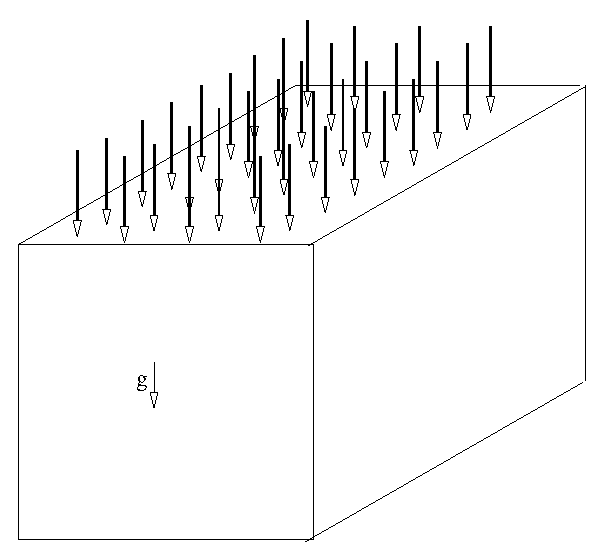
\includegraphics[scale=0.5]{M/ex_plate_model.eps}
  \end{center}
  \caption{Conceptual model of elastic foundation}
  \label{fme:cfound}
\end{figure}

The calculation area has a size of  $50m\times50m$ (length and height)
and the problem is simplified under the condition of plane strain.
The quadrilateral mesh is illustrated in Fig. \ref{fme:block},
   one corner of which is finely meshed in order that it can be used directly to
   conduct an elastic excavation simulation in a coming example.
\begin{figure}[!htb]
  \begin{center}
    \includegraphics[scale=0.3]{M/e1_mesh.eps}
  \end{center}
  \caption{Special discretization: 1150 quadrilateral elements, 1101 nodes }
  \label{fme:block}
\end{figure}
\subsubsection*{Initial and boundary conditions}
Initial conditions are not required for this problem. As for boundary conditions,
the top boundary is prescribed with a uniformly distributed pressure of $23.75MPa$. Such kind of boundary conditions
 are so called  traction boundary in the context of mechanics, they are treated as Neumann type boundary condition. More detailed boundary conditions are illustrated in Fig. \ref{fme:e1bc}.
\begin{figure}[!hbt]
  \centering
  \input{M/e1.eepic}
  \caption{Boundary conditions}
  \label{fme:e1bc}
\end{figure}
%

\subsubsection*{Material properties}
Homogeneous material properties are assumed within the whole domain. Table \ref{tme:el2d} gives the parameters.
 \begin{table}[!htb]
\centering
\begin{tabular}{lll}
\hline\hline\noalign{\smallskip}
Property & Value & Unit \\
\noalign{\smallskip}\hline\noalign{\smallskip}
Young's modulus & $25$  &GPa \\
Poisson's ratio & $0.3$             & $-$ \\
Density & $2500$             & $kg/m^3$ \\
\noalign{\smallskip}\hline\hline
\end{tabular}
\caption{Material parameters}
\label{tme:el2d}
\end{table}
%
\subsubsection*{Results}
For this simple elastic problem, we have an analytic solution given by
\begin{equation}
 \stress_{yy} = -23.75-\dens h\, \mbox[MPa]
  \label{eq:ex1_ana}
\end{equation}
where $\dens$ is the solid density and $h$ is the height from top to bottom boundary.


Fig. \mbox{\ref{fme:e1_syy} (left)} shows the distribution of vertical stress in the domain, which implies that the
 discretization error is very small. Fig. \mbox{\ref{fme:e1_syy} (right)} shows a linear variation of
   stress $\stress_{yy}$ along with height.
\begin{figure}[!thb]
  \begin{center}
  \epsfig{figure=M/e1_uy.eps,width=6cm, height=6cm}
  \epsfig{figure=M/ex1_plate_profile.eps,width=6cm, height=6cm}
  \end{center}
  \caption{Result of vertical stress, $\stress_{yy}$ (MPa). Left: domain distribution. Right: Vertical profile }
  \label{fme:e1_syy}
\end{figure}

The numerical result of $\stress_{yy}$ at the bottom boundary is \mbox{-24.97MPa}, which is very close to
 the analytic solution, $\stress_{yy}=-25.0\mbox{MPa}$. This proves the correction of the numerical scheme.


%
\subsubsection*{Benchmark deposit}
\begin{tabular}{|l|l|l|}
  \hline
  Benchmark & Problem type & Path in benchmark deposit \\
  \hline
 \emph{m\_drift} & M & benchmarks\verb \M\ \\
  \hline
\end{tabular}


%%initial stress state: given (directions), function (depth
%%dependent), isotropic (Poisson ratio 0.5)
%%
\newpage

\subsection[Excavation in homogeneous media (2D)]{Plain strain with uniform loading - Excavation in homogeneous media (2D)}
\label{sec:e2}
\subsubsection*{Problem definition}
This is the second step of the simulation described in the above
section, Section \ref{sec:el2d}. A long round tunnel is built in the rock mass and this is depicted in Fig. \ref{fme:excav}.
 The deformation due to the excavation  is simulated under the assumption of plane strain, same initial condition and materail parametrers given in Section {sec:el2d}.
\begin{figure}[!thb]
  \begin{center}
  \epsfig{figure=M/ex_plate.eps,width=7cm, height=7cm}
  \end{center}
  \caption{Excavation in rock mass }
  \label{fme:excav}
\end{figure}


\subsubsection*{Initial and boundary conditions}
The tunnel has a radius of $5m$. The released loading apprach is applied to simulate the excavation.

\subsubsection*{Results}
We use the same mesh as given in the above section to conduct the similation.
Fig. \ref{fig:e2cont} shows the distribution of vertical
displacement and and stresses in the domain after excavation.

\begin{figure}[!htb]
  \begin{center}
   %%\vspace{-2.7cm}
   \begin{minipage}[t]{0.45\textwidth}
     \begin{center}
    \includegraphics[scale=0.3]{M/ee_uy.eps}
    \centerline{Vertical displacement (m)}
    \end{center}
   \end{minipage}
  \hspace{0.02\textwidth}
   \begin{minipage}[t]{0.45\textwidth}
    \begin{center}
    \includegraphics[scale=0.3]{M/ee_sxx.eps}\\
    \centerline{Horizontal stress (MPa)}
    \end{center}
   \end{minipage}\\
  \end{center}
  \caption{State variables after excavation}
  \label{fig_modelhm}
\end{figure}

\begin{figure}[!htb]
  \begin{center}
   %%\vspace{-2.7cm}
   \begin{minipage}[t]{0.45\textwidth}
     \begin{center}
    \includegraphics[scale=0.3]{M/ee_sxy.eps}
    \centerline{Shear stress (MPa)}
    \end{center}
   \end{minipage}
  \hspace{0.02\textwidth}
   \begin{minipage}[t]{0.45\textwidth}
    \begin{center}
    \includegraphics[scale=0.3]{M/ee_syy.eps}\\
    \centerline{Vertical stress (MPa)}
    \end{center}
   \end{minipage}\\
  \end{center}
  \caption{State variables after excavation}
  \label{fig:e2cont}
\end{figure}
\subsubsection*{Benchmark deposit}
\begin{tabular}{|l|l|l|}
  \hline
  Benchmark & Problem type & Path in benchmark deposit \\
  \hline
 \emph{m\_drift} & M & benchmarks\verb \M\ \\
  \hline
\end{tabular}

\clearpage

\subsection[Excavation in heterogeneous media (2D)]{Plain strain with uniform loading - Excavation in heterogeneous media (2D)}
\label{sec:e3}
\subsubsection*{Problem definition}
Again, we analyze the deformation of the excavtion problem defined in Section \ref{sec:e2}. Contrary to homogeneous case,
  we  use function defined initial stress and assume four different material domains
 make up the geometry (Fig. \ref{fme:excav2}).
\begin{figure}[!thb]
  \begin{center}
  \epsfig{figure=M/m_drift_init.eps,width=7cm, height=7cm}
  \end{center}
  \caption{Excavation in heterogeneous rock mass }
  \label{fme:excav2}
\end{figure}


\subsubsection*{Initial and boundary conditions}
The initial stresses are assumed linearly distributed within a material domain.
 The expressions of these distribution are given in
 \begin{table}[!htb]
\centering
\begin{tabular}{llll}
\hline\hline\noalign{\smallskip}
Material & & Expression &  \\
  (Fig.  \ref{fme:excav2} ) &$\sigma_{xx}$ &$\sigma_{yy}$ &$\sigma_{zz}$  \\
\noalign{\smallskip}\hline\noalign{\smallskip}
   1 & $23.75+0.2y       $ &  $   23.75+0.2y     $   &  $     23.75+0.2y    $  \\
   2  & $24.75+0.5y       $ &  $   24.75+1.3y     $   &  $     24.75+0.5y    $ \\
   3  & $26.75+10.0x+12.0y  $ &  $  26.75+20.0x+16.0y $   &  $    26.75+10.0x+12.0y$  \\
   4  & $27.75+10.0x+14.0y $ &  $  27.75+20.0x+18.0y$   &  $   27.75+10.0x+14.0y$  \\
\noalign{\smallskip}\hline
\end{tabular}
\caption{Initial stress expression ( negative value, kPa)}
\label{tab:initialStress}
\end{table}

\subsubsection*{Material properties}
As depicted in Fig. \ref{fme:excav2}, the domain  consists of four different materials denoted
    by 1, 2, 3 and 4. Hereby, we assume only Young's modulus differs from each other of materials
    (Table \ref{tme:el2dHR}).
 \begin{table}[!htb]
\centering
\begin{tabular}{lll}
\hline\hline\noalign{\smallskip}
Property & Value & Unit \\
\noalign{\smallskip}\hline\noalign{\smallskip}
Young's modulus & {\color{red}1:}$25$, {\color{red}2:}26.0, {\color{red}3:}30.0,
   {\color{red}4:}28.0  &GPa \\
Poisson's ratio & $0.3$             & $-$ \\
Density & $2.5$             & $kg/m^3$ \\
\noalign{\smallskip}\hline\hline
\end{tabular}
\caption{Parameters}
\label{tme:el2dHR}
\end{table}

\subsubsection*{Results}

Fig. \ref{fme:exH_disp} shows the distribution of displacements after excavation.
 \begin{figure}[!thb]
  \begin{center}
  \epsfig{figure=M/ex_h_ux.eps,width=6cm, height=6cm}
  \epsfig{figure=M/ex_h_uy.eps,width=6cm, height=6cm}
  \end{center}
  \caption{Distribution of displacement (m)}
  \label{fme:exH_disp}
\end{figure}

\clearpage

Fig. \ref{fme:exH_stress} shows the distribution of stresses after excavation.
 \begin{figure}[!thb]
  \begin{center}
  \epsfig{figure=M/ex_h_sxx.eps,width=6cm, height=6cm}
  \epsfig{figure=M/ex_h_sxy.eps,width=6cm, height=6cm}
  \epsfig{figure=M/ex_h_syy.eps,width=6cm, height=6cm}
  \epsfig{figure=M/ex_h_szz.eps,width=6cm, height=6cm}
  \end{center}
  \caption{Distribution of stresses (kPa)}
  \label{fme:exH_stress}
\end{figure}

\subsubsection*{Benchmark deposit}
\begin{tabular}{|l|l|l|}
  \hline
  Benchmark & Problem type & Path in benchmark deposit \\
  \hline
 \emph{m\_drift\_init} & M & benchmarks\verb \M\ \\
  \hline
\end{tabular}
%%\subsubsection{Multiple excavation}

\clearpage

\subsection{Elastic cube (3D)}
\subsubsection*{Problem definition}
We consider deformation in a cubic domain under linearly distributed pressure (Fig. \ref{fig:brick}).
The size the domain is $1m\times1m\times1m$. The deformation is assumed being elastic.
\begin{figure}[!htb]
  \begin{center}
    \includegraphics[scale=0.3]{M/brick_l.eps}
  \end{center}
  \caption{A block with linear distributed pressure on the top surface}
  \label{fig:brick}
\end{figure}
\subsubsection*{Initial and boundary conditions}
 Normal translation on the vertical surfaces, which contains vertex A, D and
which contains vertex B, C, and on the bottom surface is restricted. On the top surface, a linear distributed
 pressure is prescribed in the manner of point-wise as:
 \begin{itemize}
   \item Vertex A: $1.0Pa$
   \item Vertex B:  $1.0Pa$
   \item Vertex C:  $0.0Pa$
   \item Vertex D:  $0.0Pa$
 \end{itemize}
The pressure at any point on the top surface is obtained by a linear interpolation before face integration.
This is done by programm automatically.
\subsubsection*{Material properties}
The material properties are homogenous with the domain and they are listed in Table \ref{tab:ecub}
 \begin{table}[!htb]
\centering
\begin{tabular}{lll}
\hline\hline\noalign{\smallskip}
Property & Value & Unit \\
\noalign{\smallskip}\hline\noalign{\smallskip}
Young's modulus & $2.0\times 10^{7}$  &Pa \\
Poisson's ratio & $0.4$             & $-$ \\
\noalign{\smallskip}\hline\hline
\end{tabular}
\caption{Material parameters of cubic domain}
\label{tab:ecub}
\end{table}
\subsubsection*{Results}
A deformed domain is depicted in Fig. \ref{fig:brick_d}, which demonstrated that the results
  are consistent with the prescribed boundary condition.
 \begin{figure}[!htb]
  \begin{center}
    \includegraphics[scale=0.4]{M/brick_l_d.eps}
  \end{center}
  \caption{Deformed cubic domain}
  \label{fig:brick_d}
\end{figure}
\subsubsection*{Benchmark deposit}
\begin{tabular}{|l|l|l|}
  \hline
  Benchmark & Problem type & Path in benchmark deposit \\
  \hline
 \emph{m\_brick\_l} & M & benchmarks\verb \M\ \\
  \hline
\end{tabular}

\clearpage

\subsection{Given deformation at the top (3D)}

\textbf{Problem definition}

A quarter of an elastic cylinder is compressed at the top. The deformation that is caused by a uniform vertical stress is given as boundary condition. The aim is to calculate the stress in $z$-direction which is caused by this deformation and to get to know the resulting deformations in each direction.

\begin{figure}[htbp]
\centering
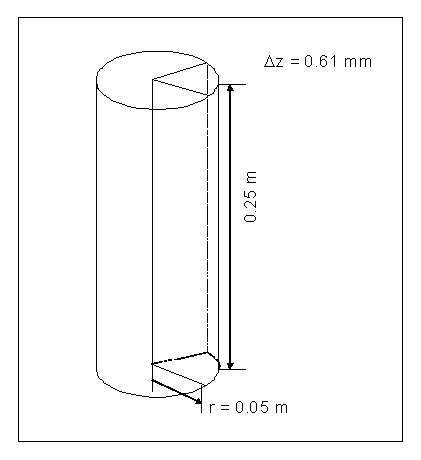
\includegraphics[width=0.4\textwidth]{M/figures/fig31.eps}
\caption{Calculation area: a quarter of a cylinder}
\label{fig31}
\end{figure}

%\newpage

\textsl{Assumptions}

\begin{tabbing}
\=xxxxxxxxxx  \=xxxxxxxxxxxxxxxxxxxxxxx \kill
\> Solid: \> homogeneous, isotropic, finite dimensions, constant deformation, \\
\> \> linear elastic material behaviour
\end{tabbing}

\textbf{Model set-up of the 3D numerical model}

For the 3-dimensional simulation the calculation area is exclusively out of a quarter of a cylinder. The model includes 4000 elements and 4947 nodes. Deformations in $x$-direction are suppressed in the $y-z$-plane. Deformations in $y$-direction are suppressed in the $x-z$-plane and deformations in $z$-direction are inhibited at the bottom of the quarter cylinder. At the top of the model a mechanical boundary condition is set with a constant displacement of 0.61~mm. The elastic deformation of the solid is not time-dependent. The used material parameters are shown in Tab. \ref{tab33}.
\begin{table}[htbp]
\centering
\begin{tabular}{|c|l|l|}
\hline
symbol & quantity & value \\
\hline
$\rho$  & density of the solid &  2.5 t$\cdot$m$^{-3}$  \\			
\hline
$E$ & Young's modulus of the solid & 7 GPa \\
\hline
$\nu$ & Poisson ratio & 0.3 \\
\hline
\end{tabular}
\caption{Material parameters}
\label{tab33}
\end{table}

\begin{figure}[htbp]
\centering
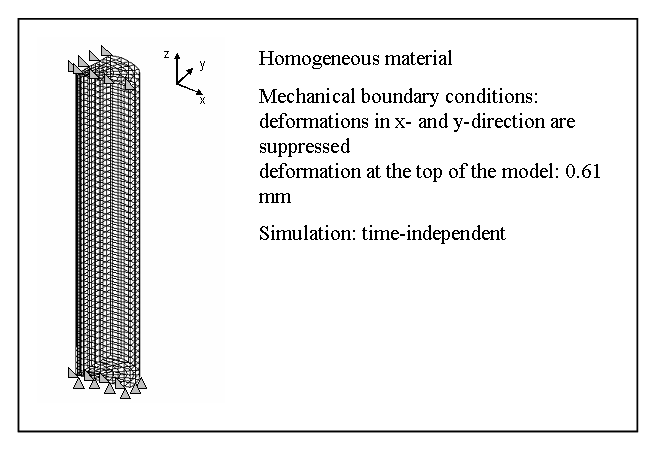
\includegraphics[width=0.5\textwidth]{M/figures/fig32.eps}
\caption{Calculation model (3D)}
\label{fig32}
\end{figure}

\newpage

\textbf{Evaluation method}

In order to solve the equations of the Hooke's law, there are some constraints that have to be considered: the stresses in $x$- and $y$-direction are equal to zero, because the body can expand into radial direction. Thus the Hooke's equations can be simplified as follows:
\begin{eqnarray}
\varepsilon_z & = &
\frac{\Delta z}{z}\,=\,\frac{1}{E}\cdot\sigma_z
\label{eq36} \\[1.5ex]
\varepsilon_x & = &
\varepsilon_x\,=\,\frac{1}{E}\cdot\left(-\nu\cdot\sigma_z\right)
\label{eq37}
\end{eqnarray}

\textbf{Results}

With the given strain in $z$-direction, the stress $\sigma_z$ is calculated by Eqn. \ref{eq36}.
\begin{displaymath}
\frac{\Delta z}{z}=\frac{-6.1\cdot 10^{-4}\,\mathrm{m}}{0.25\,\mathrm{m}}=-2.44\cdot 10^{-3}
\quad\mathrm{and}\quad
\sigma_z=-2.44\cdot 10^{-3}\cdot 7\cdot 10^{9}\,\mathrm{Pa}=
-1.71\cdot 10^{7}\,\mathrm{Pa}
\end{displaymath}

In this way, the strains in $x$- and $y$-direction are known.
\begin{displaymath}
\varepsilon_x\,=\,\varepsilon_y\,=\,
\frac{1}{7\cdot 10^{9}\,\mathrm{Pa}}\cdot
\left(-0.3\cdot-1.71\cdot 10^{7}\,\mathrm{Pa}\right)\,=\,
7.32\cdot 10^{-4}
\end{displaymath}

The numerical results meet exactly the analytical solutions. This is sketched in Fig. \ref{fig33}, where the strains and the resulting stress along a polyline from top to bottom of the quarter cylinder can be found. That means both RockFlow and GeoSys/RockFlow are able to calculate the state of stresses for the 3D elastic deformation.

\clearpage

\begin{figure}[htbp]
\centering
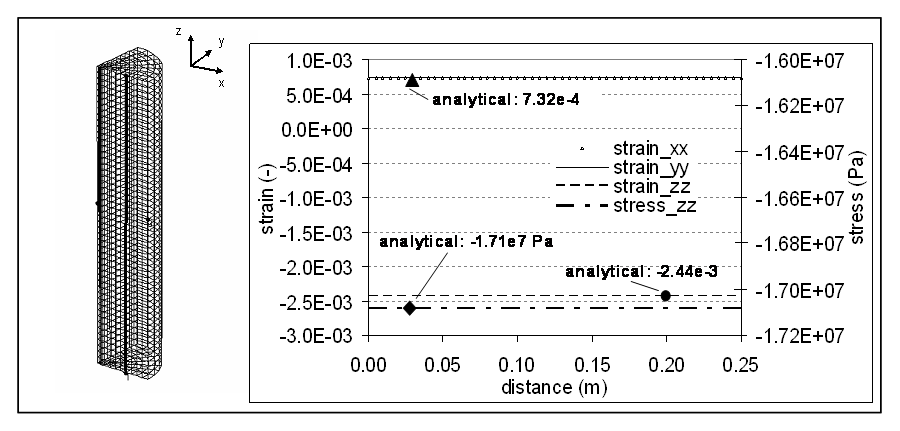
\includegraphics[width=0.9\textwidth]{M/figures/fig33.eps}
\caption{Strains and stress in $z$-direction as the result of deformation}
\label{fig33}
\end{figure}

\vskip 4.0ex

\begin{tabular}{|l|l|l|l|}
\hline
Path in the & Used code	& Used version & Date of si- \\
benchmark deposit	& & & mulation run \\
\hline	
$\backslash$M$\backslash$elastic\_deformation$\backslash$	& GeoSys/RockFlow	& RockFlow 4,	& Dec. 2007 \\
displacement$\backslash$displ\_Geosys/	& & rf4-507 & \\
RF$\backslash$m\_e\_displacement\_3Du	& & & \\
\hline	
\end{tabular}


\clearpage

\subsection{Given stress at the top (3D)}

\textbf{Problem definition}

This example is the inverse of the precedent one. The quarter cylinder is deformed by a given stress, while this time the resulting deformation is unknown. In order to check out easily whether the simulated results correspond to the analytical solutions, the value of the effective stress in $z$-direction on top of the calculation model is the same as in the above described example.

\textsl{Assumptions}

\begin{tabbing}
\=xxxxxxxxxx  \=xxxxxxxxxxxxxxxxxxxxxxx \kill
\> Solid: \> homogeneous, isotropic, finite dimensions, constant deformation, \\
\> \> linear elastic material behaviour
\end{tabbing}

\textbf{Model set-up of the 3D numerical model}

The calculation model has the same properties as the model of the precedent example. At the top of the model a load of -1.71$\cdot$10$^7$~Pa was set as constant source term. The simulation with both RockFlow and Geosys/RockFlow needs the input of the load as source term in $z$-direction at the single nodes under consideration of each element node. The input is done as single forces, not as the common stresses. The displacement boundaries are the same as in the precedent example except the $z$-displacement on the top of the model. The used material parameters are shown in Tab. \ref{tab33}.

%\newpage

\textbf{Results}

The analytical solution and results are identical to the previous example. The calculated displacement as a result of the constant load on the top amounts to 6.1$\cdot$10$^{-4}$~m. The numerical results that are shown in Fig. \ref{fig34} meet the analytical solutions well.

\begin{figure}[htbp]
\centering
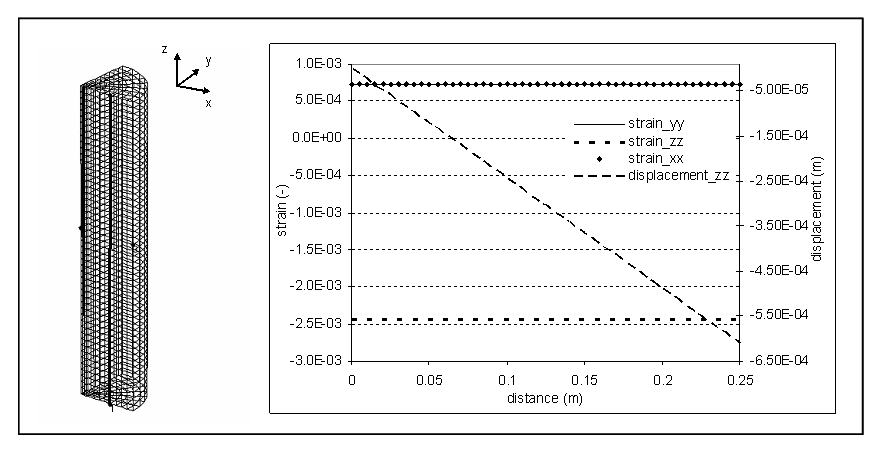
\includegraphics[width=0.9\textwidth]{M/figures/fig34.eps}
\caption{Strains and displacement in $z$-direction}
\label{fig34}
\end{figure}

\begin{tabular}{|l|l|l|l|}
\hline
Path in the & Used code	& Used version & Date of si- \\
benchmark deposit	& & & mulation run \\
\hline
$\backslash$M$\backslash$elastic\_deformation$\backslash$	& GeoSys/RockFlow	& RockFlow 4,	& Dec. 2007 \\
stress$\backslash$stress\_Geosys/RF$\backslash$	& & rf4-507 & \\
m\_e\_stress\_3Du	& & & \\
\hline	
\end{tabular}


\clearpage

\subsection{Lubby1: Nonlinear model}
\label{subsec:lubby1}
The Lam{\'{e}} constants defined for Hooke's fourth-order elastic material tensor (\ref{eq:hook}) can be expressed by the Young's modulus $E$, the Poisson's ratio $\nu$ and the shear modulus $G$ (so-called {\sl enginering constants}) which can be obtained experimentally.
\begin{eqnarray}
\mu     & = & \ttfrac{E}{2(1+\nu)}\,=\,G \\[1.5ex]
\lambda & = & \ttfrac{E\nu}{(1+\nu)(1-2\nu)}\,=\,\ttfrac{2G\nu}{(1-2\nu)}
\end{eqnarray}

In many technical applications considering small strains, the elastic material parameters are assumed to be constant, and the stress-strain curves are nearly linear. However, the typical response of certain geological materials to monotonic loading (without load reversal) shows a nonlinear stress-strain behavior. Considering only elastic effects during load application, Hooke's law cannot be used to describe the observed material properties. Therefore, so-called pseudo-elastic constitutive models are frequently used for the analysis of nonlinear stress-strain curves, particularly in soil and rock mechanics. In a generalized manner, they are based on the assumption of an explicit stress-strain relation considering a stress- and strain-dependent material matrix:
\begin{equation}
\mio{\sigma}{}{}\,=\,\fourtens{\mathcal{C}}(\mio{\sigma}{}{},\mio{\varepsilon}{}{})\ccdot\mio{\varepsilon}{\mathrm{e}}{}\,.
\label{elasticity_nonlin}
\end{equation}

Based on the so-called {\sl Lubby1} model (cf. \cite{Lux:1984}), a nonlinear elastic approach with strain-dependent Young's modulus
\begin{equation}
E(\varepsilon_{\mathrm{v}})\,=\,\frac{E_0}{1+a\,\varepsilon_{\mathrm{v}}^n}
\label{lubby1_ev}
\end{equation}
but constant Poisson's ratio is proposed. Here, $\varepsilon_{\mathrm{v}}$ is the equivalent strain, and $E_0$, $a$ as well as $n$ are material parameters . The equivalent strain is defined by
\begin{equation}
\varepsilon_{\mathrm{v}}\,=\,
\sqrt{\frac{2}{3}\,\mio{\varepsilon}{\mathrm{e}}{}\ccdot\mio{\varepsilon}{\mathrm{e}}{}}\,.
\end{equation}

\subsubsection*{Problem definition}

Triaxial short-term compression under axisymmetric conditions is carried out to verify the nonlinear elastic isotropic material model (modified Lubby1 approach). For the calculation, the cross-section of a cylindrical sample with a radius of 30~mm and a height of 120~mm is studied. The loading in principal axes includes a radial pressure as well as an axial displacement, and is realized in two steps. It is resulting in a homogeneous stress-strain state. Details of the model (geometry, mesh, boundary conditions) according to K.-H. Lux and F. Werunsky (unpublished report, 2008) are presented in Fig.~\ref{triax_model_lubby1}.

\begin{figure}[!htb]
\begin{center}
\includegraphics[width=0.2\textwidth]{M/figure/svv_model.eps}
\hspace*{10.0ex}
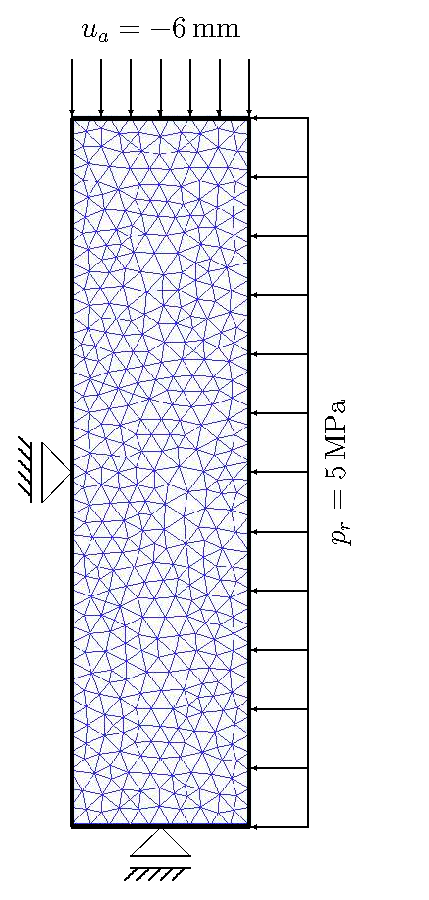
\includegraphics[width=0.25\textwidth]{M/figure/svv_mesh.eps}
\end{center}
\caption{Triaxial compression of a cylindrical sample. Axisymmetric model. Left: Geometry. Right: Finite element grid and boundary conditions.} 
\label{triax_model_lubby1}
\end{figure}

\begin{figure}[!htb]
\begin{center}
\includegraphics[width=0.6\textwidth]{M/figure/svv_loadhistory.eps}
\end{center}
\caption{Triaxial compression of a cylindrical sample. Loading history for short-term experiments. Radial casing pressure (stress rate $\dot{p}{}_r=0.25$\,MPa$\cdot$s$^{-1}$) with subsequent axial displacement (strain rate $\dot{\varepsilon}{}_a=3.47\cdot 10^{-5}$\,s$^{-1}$).} 
\label{triax_loadhist_lubby1}
\end{figure}

\subsubsection*{Initial and boundary conditions}

Initial conditions do not have to be given for the problem under consideration. As the bottom edge is fixed in vertical direction, the left-hand edge is fixed in horizontal direction for symmetry reasons (axis of rotation). On the right-hand edge initially a radial casing pressure of 5~MPa is applied within 20~seconds with a constant stress rate. While keeping constant this radial pressure, a subsequent stroke-driven axial compressive loading is applied within the following 1\,440~seconds with a constant strain rate. The maximum axial displacement is 6~mm which corresponds to a 5\% reduction of the sample's height (for the complex loading history cf. Fig.~\ref{triax_loadhist_lubby1}).

\subsubsection*{Material properties}
 
The material parameters referring to the modified Lubby1 relation~(\ref{lubby1_ev}) are summarized in Tab.~\ref{matpar_lubby1}. Within this context, the initial Young's modulus and the Poisson's ratio are close to values known for rock salt.
 
\vskip 3.0ex
 
\begin{table}[!htb]
\centering
\begin{tabular}{lll}
\hline\hline\noalign{\smallskip}
Property & Value & Unit \\
\noalign{\smallskip}\hline\noalign{\smallskip}
Poisson's ratio $\nu$             & 0.335   & --  \\
initial Young's modulus $E_0$     & 21\,400 & MPa \\
factor $a$ in (\ref{lubby1_ev})   & 2\,750  & --  \\
exponent $n$ in (\ref{lubby1_ev}) & 1.0     & --  \\
\noalign{\smallskip}\hline\hline
\end{tabular}
\caption{Material parameters}
\label{matpar_lubby1}
\end{table}

\subsubsection*{Results}

The representation of the axial stress vs. the axial strain in Fig.~\ref{triax_res_lubby1} shows on exemplarily chosen material parameters the noticeable difference between the linear (Hooke's model) and the nonlinear (modified Lubby1 model) elastic models even at small strains. Within the contect of the studied case, the stress response will be overestimated by a multiple using the linear Hooke's law. 

\clearpage

\begin{figure}[!htb]
\begin{center}
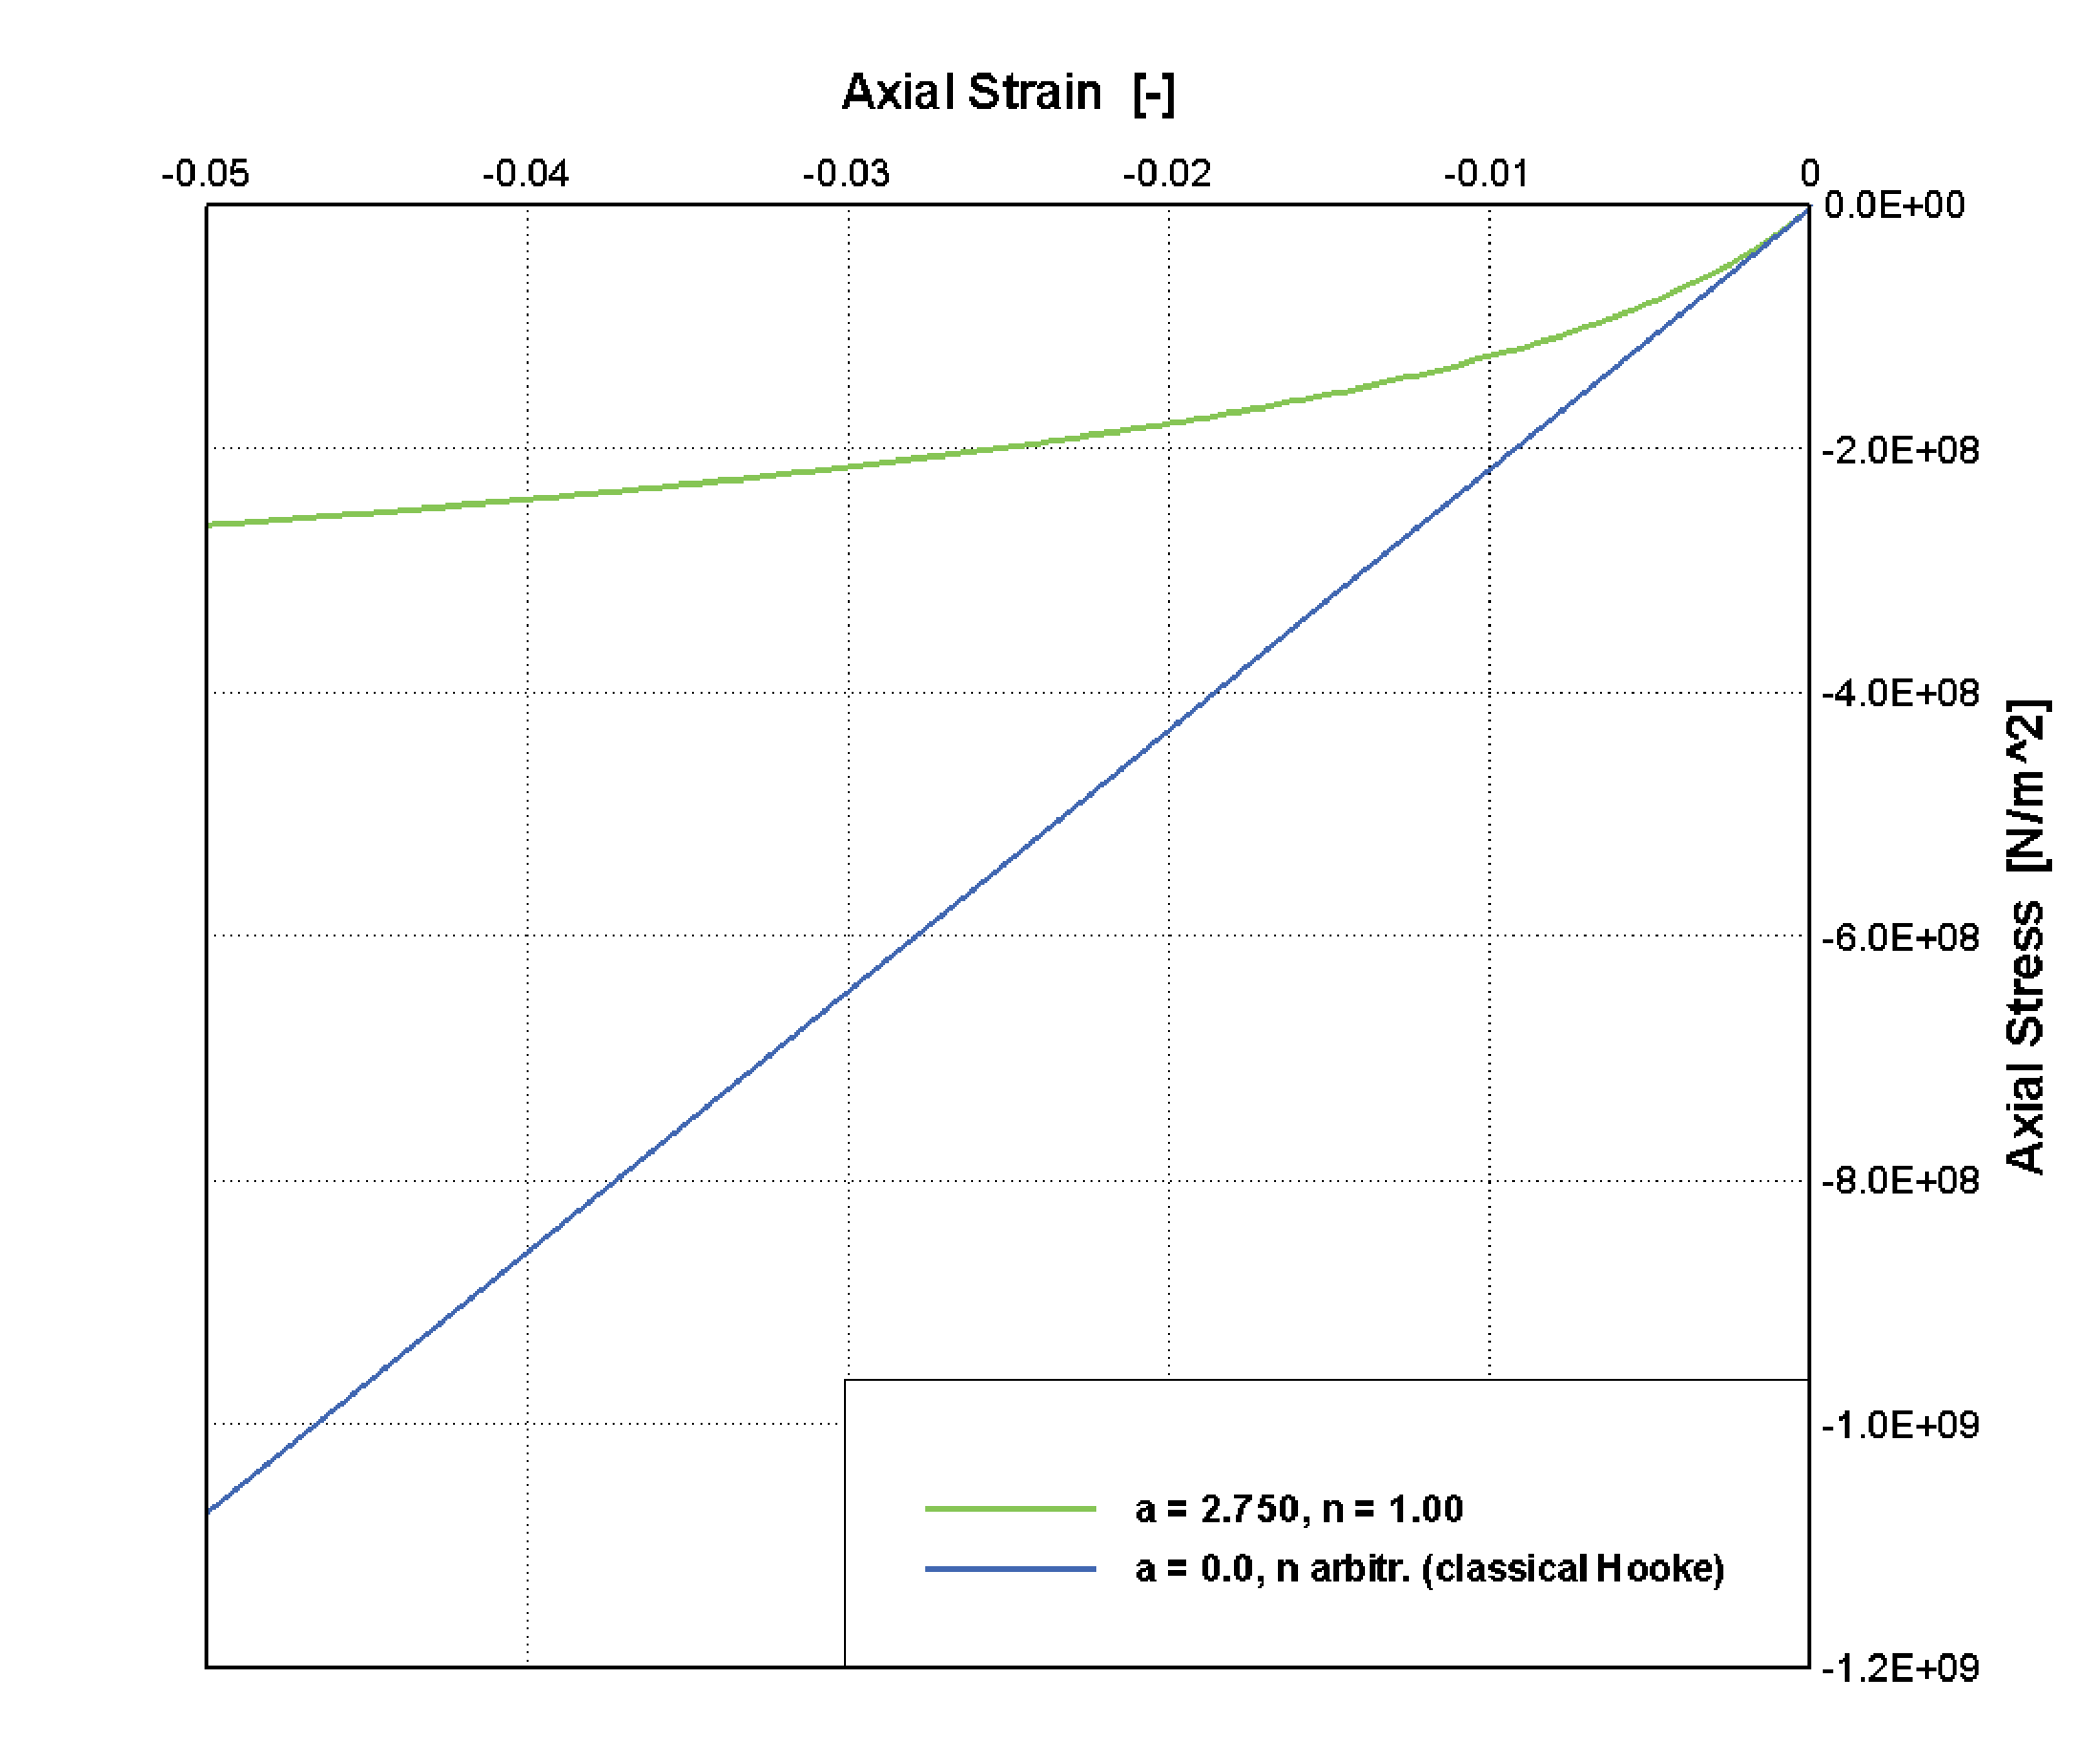
\includegraphics[width=0.6\textwidth]{M/figure/svv_e_stress_strain_hooke_lubby1m.eps}
\end{center}
\caption{Triaxial compression of a cylindrical sample. Stress-strain curves regarding the axial load response. Comparison of linear elastic (Hooke) and nonlinear elastic (modified Lubby1~(\ref{lubby1_ev})) material models.} 
\label{triax_res_lubby1}
\end{figure}

\vskip 4.0ex

\subsubsection*{Benchmark deposit}

\begin{tabular}{|l|l|l|}
  \hline
  Benchmark & Problem type & Path in benchmark deposit \\
  \hline
 \emph{m\_triax\_lubby1} & M & benchmarks\verb \M\ \\
  \hline
\end{tabular}





\include{M/elasticity_transiso}

\section{Excavation in homogeneous media (3D)}
%\label{sec:e3d}
\subsubsection*{Problem definition}
A long round tunnel is build in the rock mass. The tunnel is 9 m lang and its radius is 0.33 m. We analyze the distribution of displacement and stresses after the excavtion. Different with the above section there is no plain stain at top the model. Fig. \ref{fme:e3d_g}

\begin{figure}[!htb]
  \begin{center}
    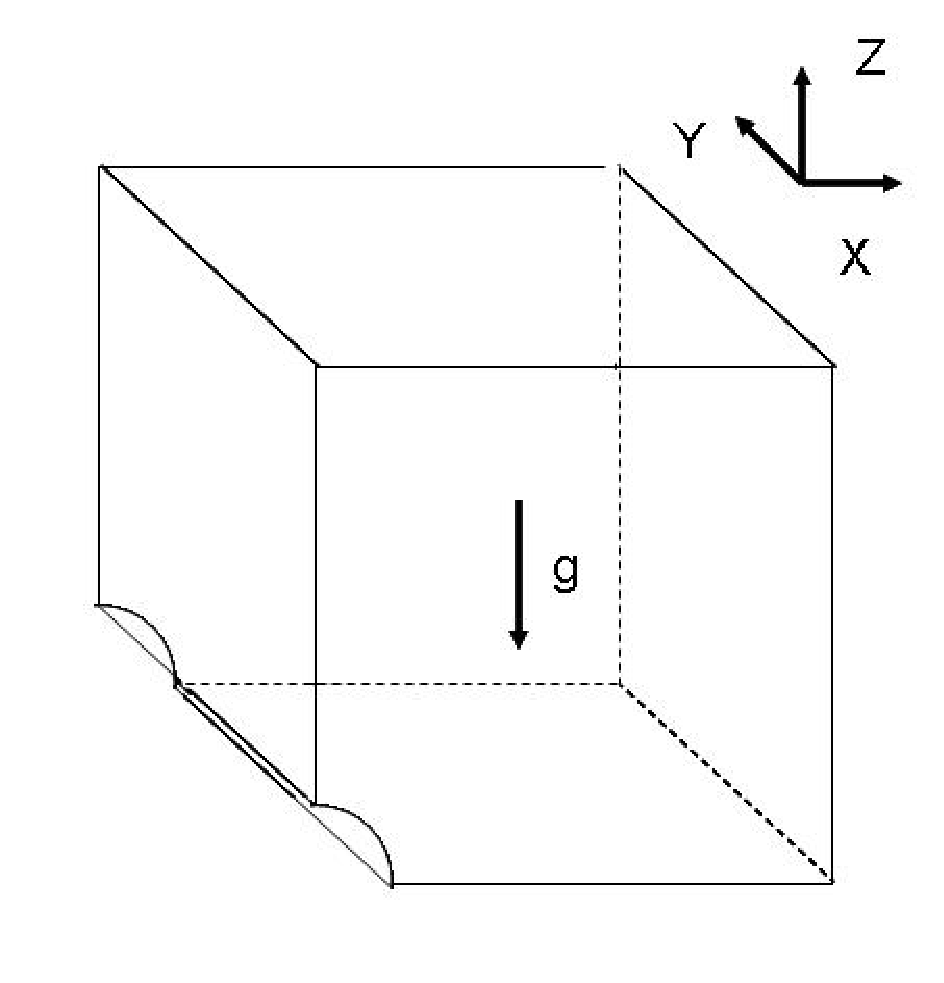
\includegraphics[scale=0.40]{M/e3d_g_model.eps}
  \end{center}
  \caption{Conceptual model of elastic foundation}
  \label{fme:e3d_g}
\end{figure}


\subsubsection*{Initial and boundary conditions}
The initial conditions are not required in this case. More detailed boundary conditions are illustrated in Fig. \ref{fme:e3d_g_bc}.
\begin{figure}[!hbt]
  \begin{center}
    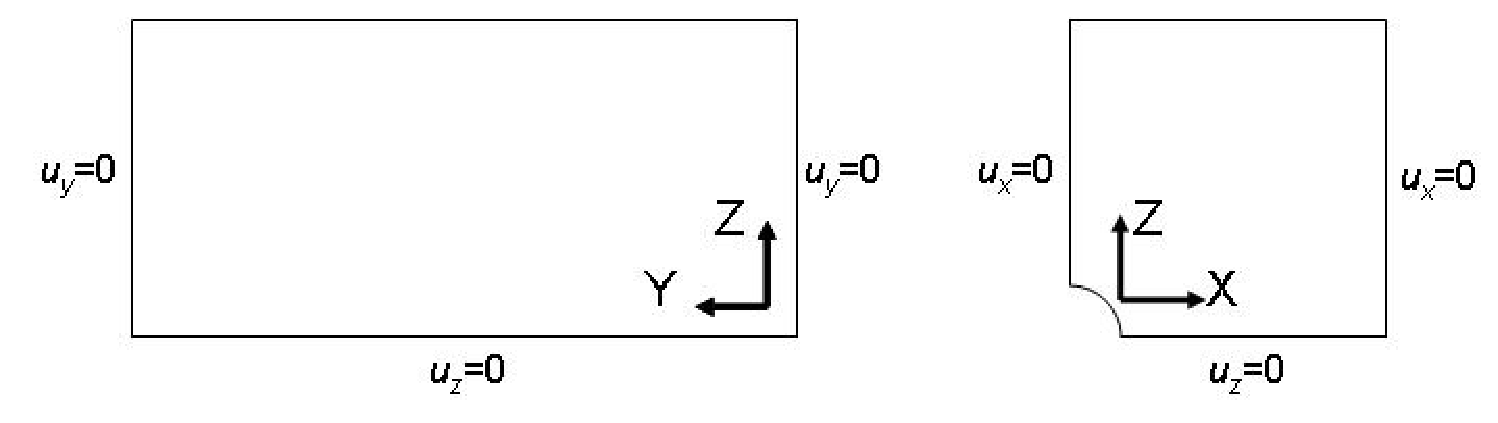
\includegraphics[scale=0.5]{M/e3d_g_bc.eps}
  \end{center}
  \caption{Boundary conditions}
  \label{fme:e3d_g_bc}
\end{figure} 
 

\subsubsection*{Material properties}

 \begin{table}[!htb]
\centering
\begin{tabular}{lll}
\hline\hline\noalign{\smallskip}
Property & Value & Unit \\
\noalign{\smallskip}\hline\noalign{\smallskip}
Young's modulus & $8$ & GPa \\
Poisson's ratio & $0.2$ & $-$ \\
Density & $2500$ & $kg/m^3$ \\
\noalign{\smallskip}\hline\hline
\end{tabular}
\caption{Parameters}
\label{tme:e3d_prop}
\end{table}

\subsubsection*{Results}
Fig. \ref{fme:e3d_disp} and \ref{fme:e3d_str} show the distribution of displacements and stresses after excavation. 

 \begin{figure}[!thb]
  \begin{center}
  \epsfig{figure=M/e3d_uz.eps,width=6cm, height=6cm}
  \epsfig{figure=M/e3d_ux.eps,width=6cm, height=6cm}
  \end{center}
  \caption{Distribution of displacement (m)}
  \label{fme:e3d_disp}
\end{figure}

\clearpage

 \begin{figure}[!thb]
  \begin{center}
  \epsfig{figure=M/e3d_szz.eps,width=6cm, height=6cm}
  \epsfig{figure=M/e3d_sxx.eps,width=6cm, height=6cm}
  \end{center}
  \caption{Distribution of stresses (Pa)}
  \label{fme:e3d_str}
\end{figure}

Fig. \ref{fme:e3d_diag} shows the radiral and tangential stresses in the X and Z direction. The results are compared to values obtained with FLAC3D version 3.10 and they are well mathed.

 \begin{figure}[!thb]
  \begin{center}
  \epsfig{figure=M/e3d_hori_diag.eps,width=6cm, height=6cm}
  \epsfig{figure=M/e3d_ver_diag.eps,width=6cm, height=6cm}
  \end{center}
  \caption{Distribution of stresses (Pa)}
  \label{fme:e3d_diag}
\end{figure} 

\subsubsection*{Benchmark deposit}

\begin{tabular}{|l|l|l|}
  \hline
  Benchmark & Problem type & Path in benchmark deposit \\
  \hline
 \emph{3d\_excav} & M & benchmarks\verb \M\excavation\3D_EX \\
  \hline
\end{tabular}

\section{Elasto-plasticity}

Plasticity is a property of a material to undergo a non-reversible change of shape in response to an applied force. During the elasto-plastic deformation, the onset of plasticity is determined by a yield criterion and post-yield deformation is governed by the yield criterion and a plastic potential. To illustrate features of elasto-plasticity deformation, we consider a uniaxial test of stress depicted in Fig. \ref{fig:uniax_test}.

\begin{figure}[!htb]
  \centering
  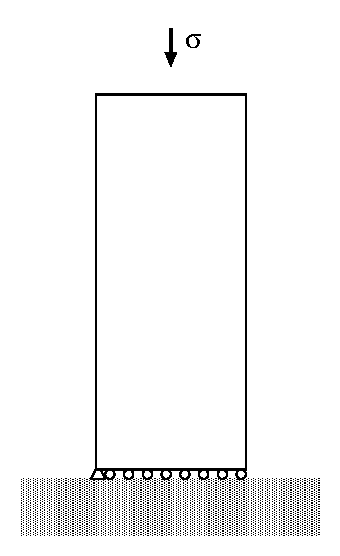
\includegraphics[scale=0.6]{M/figure/uniaxial.eps}
  \caption{Uniaxial test }
  \label{fig:uniax_test}
\end{figure}

This means only one direction has non-zero stress and strain,e.g $\stress=\sigma_{yy}$ and $\strain=\gamma_{yy}$.
Different material exhibits different elasto-plastic behavior. Fig. \ref{fig:uniax_lp} depicts a typical

\begin{figure}[!htb]
  \centering
  \input{M/figure/plast.eepic}
  \caption{Stress-strain curve of 1D problems }
  \label{fig:uniax_lp}
\end{figure}

stress-strain curve of the uniaxial test. If load $\stress$ is gradually increased, a corresponding point in $(\stress, \strain)$ plane are moving from 0 to A. Up to A, stress reaches a value $\Stress_0$, so called yield stress. If the load is removed gradually before its reaches the yield value, the point follows the line from A to 0. On the other hand, if the load is continually increased after stress is bigger than   $\Stress_0$, the material experiences plastic deformation. Assuming the curve is extended from A to B during load acting. If we remove the load gradually, the point  will not take the way its from, i.e. from B to A to 0. On the contrary, it will move from B to C linearly. Furthermore, if the load is applied again, the point will take the path from \mbox{C $\longrightarrow$ B $\longrightarrow$ D}.

This implies that: i) The unloading is elastic and there is still strain $\strain^p$ left after the load being removed,
Therefore, the plastic deformation is irreversible; ii) The strain is admissible to be decomposed into several
components, e.g. $\Stra=\Stra^e+\Stra^p$; iii) The relationship of stress-strain is history dependent curve.  Based on the last point and the  Hook's law, the constitutive equation for the 1D deformation problem can be described as

\begin{eqnarray}
\sigma_{yy}=E\varepsilon_{yy}^e=E(\varepsilon_{yy}-\varepsilon_{yy}^p)
\label{eqn:constitu_M_1D}
\end{eqnarray}

where $E$ is so called Young's modulus. If the stress-strain is monotonic increasing after yielding, the material shows hardening behavior. For some porous media, softening  behavior may be observed and its stress-strain curve looks like what depicted in Fig. \ref{fig:uniax_lp1}.

\begin{figure}[!htb]
  \centering
  \input{M/figure/plastics.eepic}
  \caption{Softening }
  \label{fig:uniax_lp1}
\end{figure}

For the constitutive equation, the case of more than one direction have non-zero stress and strain are much more complicated. A yield function $\yieldf$ and a plastic potential $\plsp$ are introduced to establish a constitutive equation. Normally, the variables of the two functions are the first, second or third stress invariant $\sivi$, $\sivii$ or $\siviii$. If we cast the yield functions to the principal stress space, we get the yield surfaces. Fig. \ref{fig:yieldsfc} depticts three typical yield surfaces of porous media.

\begin{figure}[!htb]
  \begin{center}
   \begin{minipage}[t]{0.48\textwidth}
     \begin{center}
    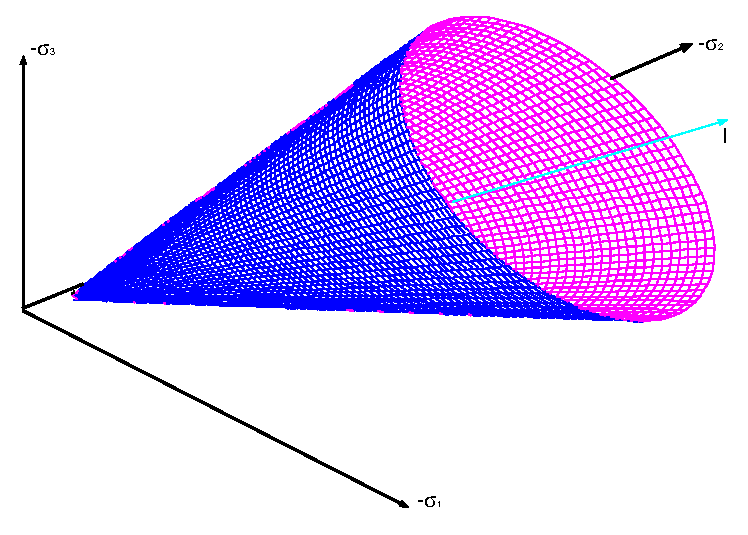
\includegraphics[scale=0.28]{M/figure/yieldsfc_dp.eps}
    \centerline{(Drucker-Prager)}
    \end{center}
   \end{minipage}
   \hspace{0.02\textwidth}
   \begin{minipage}[t]{0.48\textwidth}
    \begin{center}
    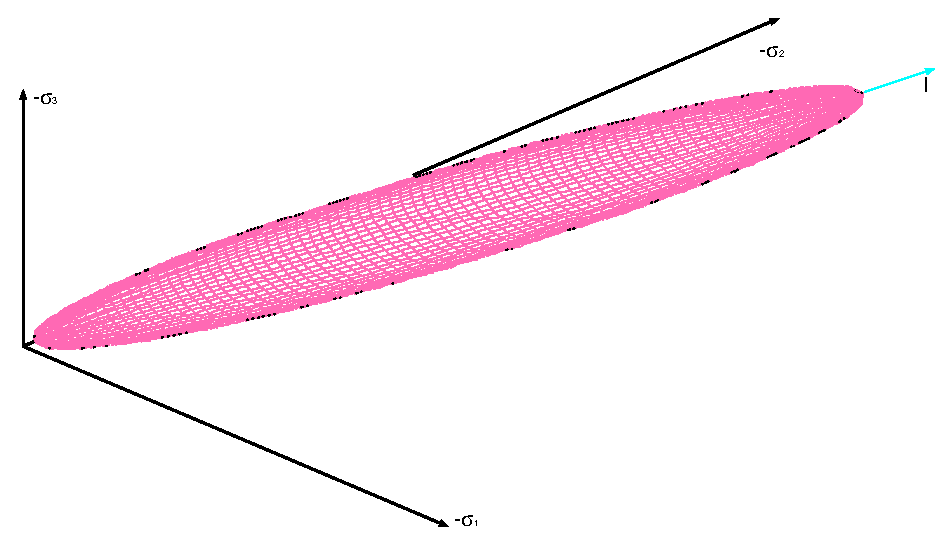
\includegraphics[scale=0.28]{M/figure/yieldsfc_cam.eps}\\
    \centerline{(Cam-Clay)}
    \end{center}
   \end{minipage}\\
   %
   \begin{minipage}[t]{0.48\textwidth}
     \begin{center}
    \includegraphics[scale=0.28]{M/figure/yieldsfc_wm.eps}
    \centerline{(Single yield surface)}
    \end{center}
   \end{minipage}
  \end{center}
  \caption{Yield surface}
  \label{fig:yieldsfc}
\end{figure}

If the stress path of any point locates inside the surface, the point undergoes elastic deformation. Otherwise, the stress status is determined by the Kuhn-Tucker criterion for the loading or unloading:

\begin{eqnarray}
\label{kuhn_tucker}
\quad \dot{\yieldf} \leq 0, \,\, \dot{ \PlasticParameter}\,{\yieldf} = 0,\,\mbox{or},\,  \dot{ \PlasticParameter} \geq 0
\end{eqnarray}

is then used to check the yield status.

Since the stress path in plastic deformation is history dependent, we describe the constitutive equations in the sense of increment of stress and strain.
Considering the generalized Hook's law (\ref{eq:hook}),  the relationship of incremantal stress  tensor $d \Stress$ and incremantal strain tensor $d \Stra$ the relationship of
stress and strain obeys the generalized Hook's law:

\begin{eqnarray}
d\Stress
= {\mathbf D} d\Stra^e=
{\mathbf D} (d\Stra-d\Stra^p)
\label{eq:ghook}
\end{eqnarray}

From the definition of plastic potential surface $\plsp$, and
normality law, it is possible to express the generalized plastic
strain increment if the potential surface is smooth. Since
$d\Stra^p$ lies parallel to the normal to $\plsp$ at $\Stress$, we
may write

\begin{eqnarray}
d\Stra^p =d \PlasticParameter \frac{\partial \plsp}{\partial \Stress}
\label{eqn:flowrule}
\end{eqnarray}

where $d \PlasticParameter$ is non-negative factor, plastic
multiplier. Equaion (\ref{eqn:flowrule}) is so clalled flow rule. Hence, the general elasto-platic constitutive equation is given by

\begin{eqnarray}
d\Stress
= {\mathbf D} d\Stra^e=
{\mathbf D} (d\Stra-d \PlasticParameter \frac{\partial \plsp}{\partial \Stress})
\label{eq:constitu_m}
\end{eqnarray}.

The flow rule is associative if $\yieldf\equiv\plsp$. Otherwise, it is non-associative. Typical plastic models, i.e. yield  functions and plastic potentials are described below.

\textit{Drucker-Prager model}

This model is a function of the two stress invariants and hardening parameter. Its yield function takes the form

\begin{eqnarray}
\yieldf (\Stress, \kappa) =\left\Vert{\devS} \right\Vert+\alpha\sivi-y(\kappa)=0 \\
\plsp (\Stress, \kappa) =\left\Vert{\devS} \right\Vert+\beta \sivi-y(\kappa)=0
\label{eqn:dp}
\end{eqnarray}

where $\alpha$ is a coefficient related to the internal frictional angle, $y(\kappa)$ is the yield stress depending on the hardening parameter.

\textit{Cam-Clay model}

Similar to the Drucker-Prager model, the Cam-Clay model is a funtion of both of the first and the second stress invariants. The generalized Cam-Clay model reads:

\begin{eqnarray}
\yieldf=q^2+M^2\pm(\pm-\pm_{cn})=0
\label{eqn:cc}
\end{eqnarray}

where $q=\sqrt{3/2}=\left\Vert {\devS} \right\Vert$, $\pm=\sivi/3$ the mean stress, $M$ is the slope of the critical state line in a $q-\pm$ digram and $\pm_{cn}$ is the isotropic preconsolidation pressure. The rate of $\pm_{cn}$ is given by

\begin{eqnarray}
{\frac{\mathrm d\, \pm\phantom{^-_-}}{\mathrm d\,  \epsilon^p_v}}=\frac{(1+e)\pm}{\lambda_c-\kappa_c}
\label{eqn:cc_pcn}
\end{eqnarray}

with $e$ the void ratio, $\epsilon^p_v$ the volume plastic strain, $\lambda_c$ the virgin compression index and $\lambda_c$  the swelling/recompression index.

The model also describes the nonlinear elastic behavior of the clay-like media before plastic yielding occurs, in which the bulk modulus $K$ is dependent of stress status as

\begin{eqnarray}
K=\frac{1+e}{\kappa_c}\pm=0
\label{eqn:cc_K}
\end{eqnarray}

with $\mu=3(1-2\nu)K/(2(1+\nu))$.

%-------------------------------------------------------------------------
\subsection{Plastic plate - von Mises plasticity (2D)}

\subsubsection*{Problem definition}

This is a typical plane strain benchmark for von Mises plasticity,
which is defined in \cite{SteEtAl:03}. We first analyze this example
to compare the behavior of two approaches on pure plastic
deformation problems. In the present simulation, a  quarter of plate
is taken due to the symmetry of the problem. The model set-up is
depicted in Fig. \ref{ex1_model}. The radius of the hole is 10$mm$.
Two points as point 1 and point 2 are specified to monitor the
evolution of variables. Point 1 is at  one third of the distance
from point 3 to point 4.

\begin{figure}[!htb]
\centering
    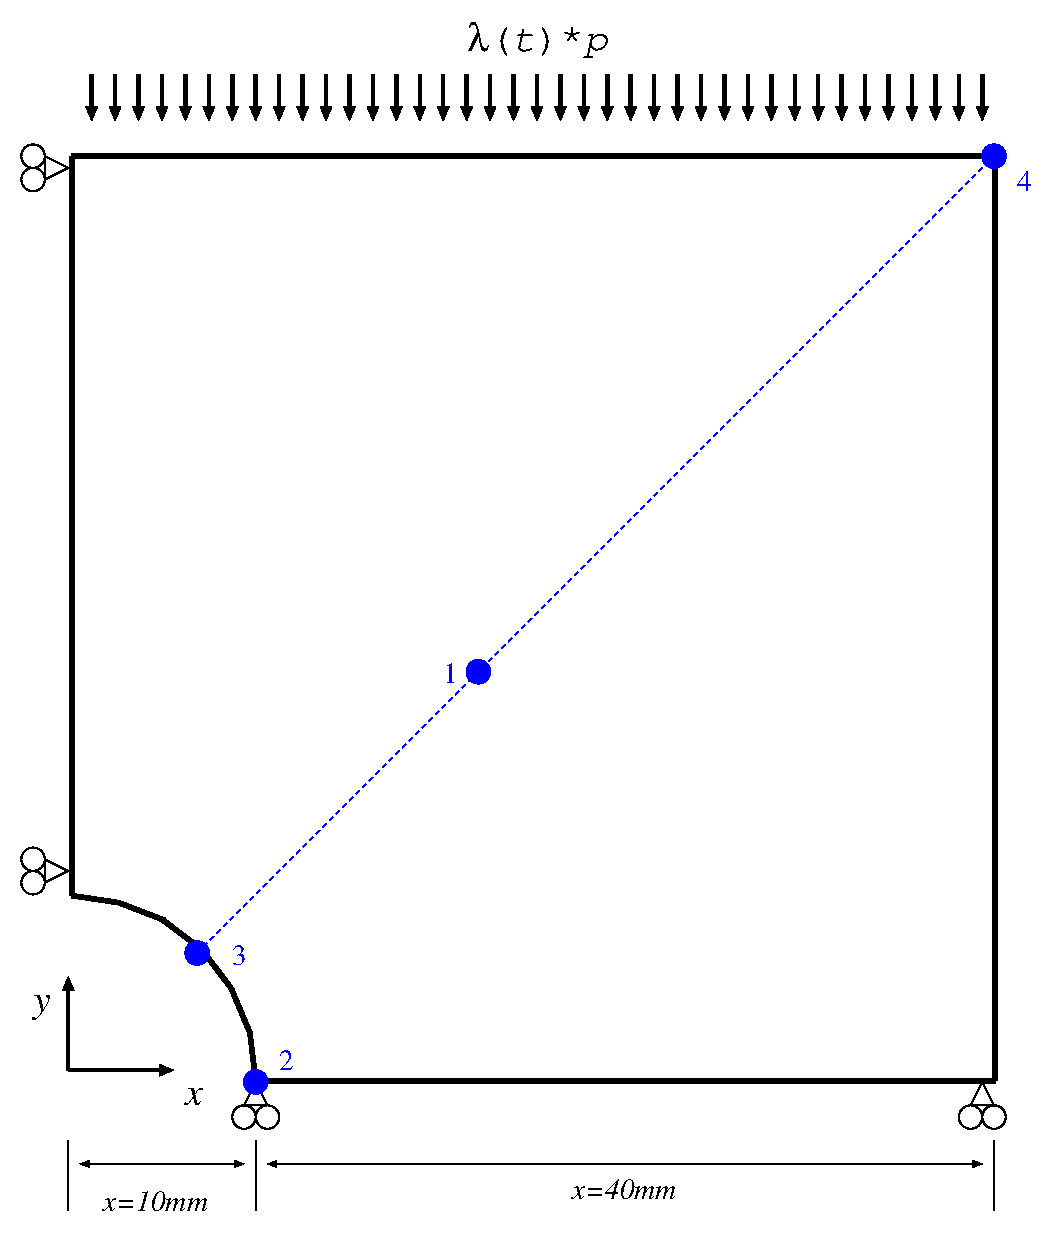
\includegraphics[scale=0.3]{M/ex1_model.eps}\\
   \caption{Stretched steel plate with a hole: one quarter}
  \label{ex1_model}
\end{figure}

\subsubsection*{Boundary conditions}

Traction boundary condition, $p=100N/mm^2\lambda(t)$  is
prescribed on the top with $\lambda(t)$, the time dependent scaling
factor. The case of  cycling loading is investigated with a scaling
function depicted in Fig. \ref{ex1_load}, in which,
$\lambda_{max}=4.1$.

\begin{figure}[!thb]
\centering
    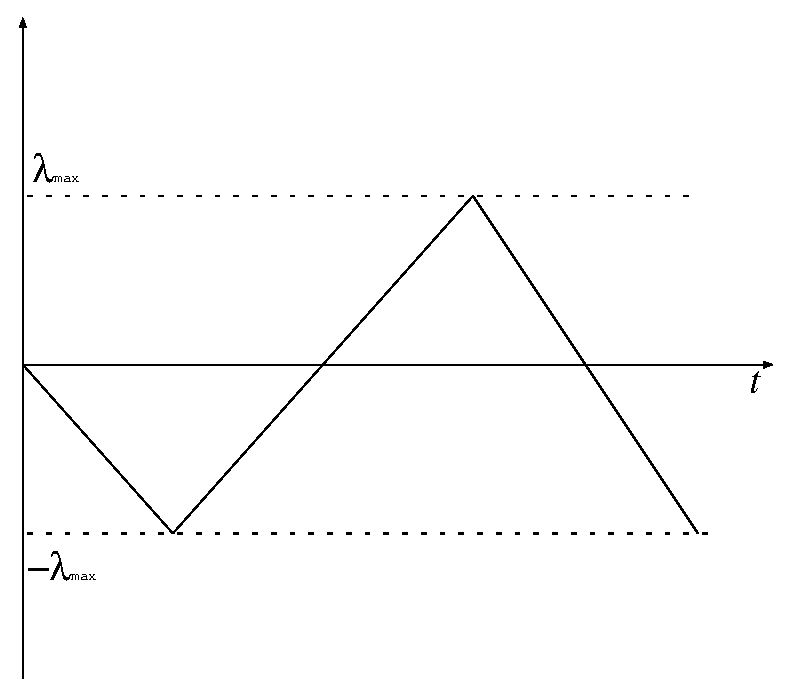
\includegraphics[scale=0.5]{M/ex1_load.eps}\\
   \caption{Time dependent load factor}
  \label{ex1_load}
\end{figure}

The domain is triangulated as depicted in Fig. \ref{ex1_mesh}.

\begin{figure}[!htb]
\centering
    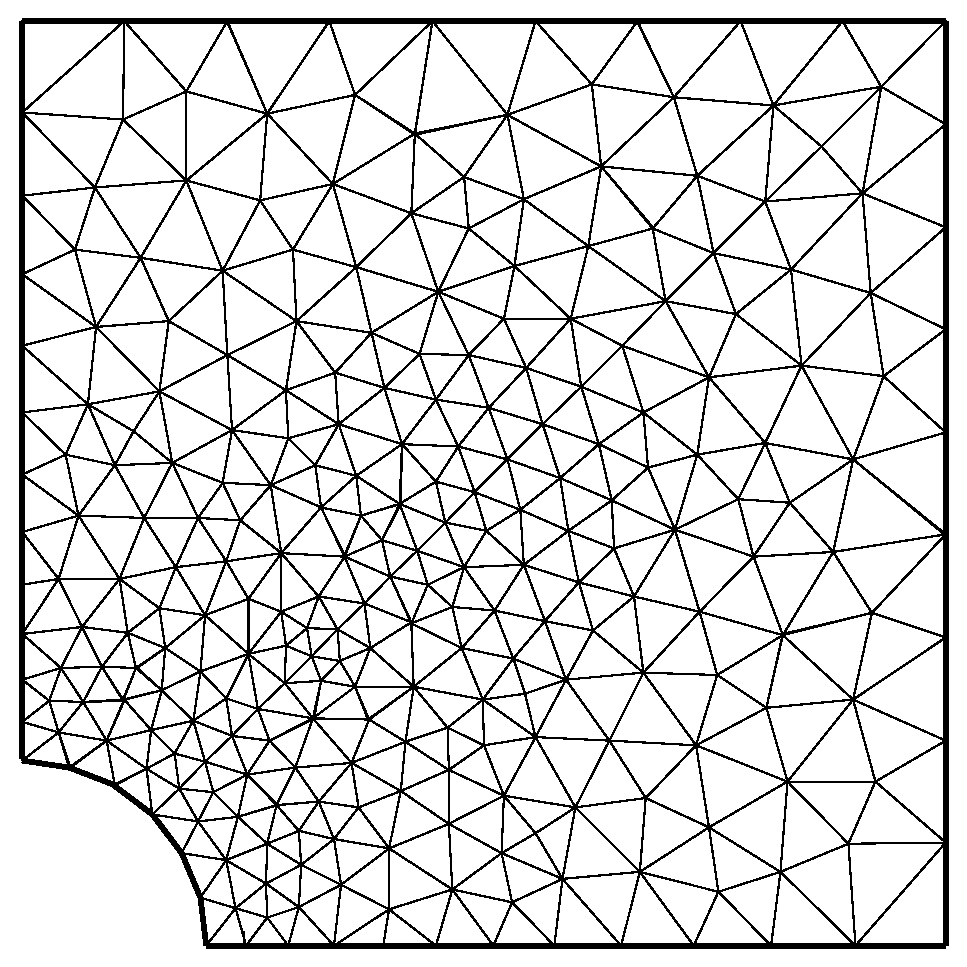
\includegraphics[scale=0.3]{M/ex1_mesh_gfem.eps}\\
   \caption{Mesh: 269 nodes and 484 elements}
  \label{ex1_mesh}
\end{figure}

\subsubsection*{Material properties}

The domain is assumed in homogeneous state. Table \ref{ex1_table1}
gives the material parameters\cite{SteEtAl:03}.

\begin{table}[!thb]
\centering
\caption{Material properties}
\label{ex1_table1}
\begin{tabular}{lll}
\hline\hline\noalign{\smallskip}
Property & Value & Unit \\
\noalign{\smallskip}\hline\noalign{\smallskip}
Young's modulus & $206900$  & $N/mm^2$ \\
Poisson's ratio & $0.29$       & $-$ \\
Initial yield stress & $450$       & $N/mm^2$ \\
Hardening modulus & $0.0$       & $kPa$ \\
\noalign{\smallskip}\hline\hline
\end{tabular}
\end{table}

\subsubsection*{Results}

The loading takes 60 steps with constant increment of
$\lambda_{max}/10$.  The similar distribution of plastic strain and
vertical stain given in Fig.\ref{ex2_cont1} shows implies the
behavior of von Mises plasticity.

%Contour plot
\begin{figure}[!thb]
  \begin{center}
   \begin{minipage}[t]{0.48\textwidth}
     \begin{center}
    \includegraphics[scale=0.28]{M/ex1_pls_4.1.eps}
    \centerline{(Plastic strain)}
    \end{center}
   \end{minipage}
   \hspace{0.02\textwidth}
   \begin{minipage}[t]{0.48\textwidth}
    \begin{center}
    \includegraphics[scale=0.28]{M/ex1_strain_yy_4.1.eps}\\
    \centerline{(Vertical strain)}
    \end{center}
   \end{minipage}\\
   %
  \end{center}
  \caption{Distribution of plastic strain and vertical strain at $\lambda_{max}/10$}
  \label{ex2_cont1}
\end{figure}

The evolution of horizontal displacements at point 1 and point 2
along with periodic load factor $\lambda (t)$ are shown on Fig.

\ref{ex2_loadp}.
\begin{figure}[!htb]
  \begin{center}
   \begin{minipage}[t]{0.48\textwidth}
     \begin{center}
    \includegraphics[scale=0.28]{M/ex1_load_v_ux_p1.eps}
    \centerline{(Point 1)}
    \end{center}
   \end{minipage}
   \hspace{0.02\textwidth}
   \begin{minipage}[t]{0.48\textwidth}
    \begin{center}
    \includegraphics[scale=0.28]{M/ex1_load_v_ux_p2.eps}\\
    \centerline{(Point 2)}
    \end{center}
   \end{minipage}\\
   %
  \end{center}
  \caption{Evolution of horizontal displacement vs load factor}
  \label{ex2_loadp}
\end{figure}

\subsubsection*{Benchmark deposit}
\begin{tabular}{|l|l|l|}
  \hline
  Benchmark & Problem type & Path in benchmark deposit \\
  \hline
 \emph{m\_mises} & M & benchmarks\verb \M\ \\
  \hline
\end{tabular}

%-------------------------------------------------------------------------
\subsection[Plastic plate - Drucker-Prager plasticity (2D)]{Plastic plate - Drucker-Prager plasticity, enhanced strain element (2D)}

\subsubsection*{Problem definition}

In this application, we analyze a plane strain biaxial failure
de\-for\-ma\-tion problem with triangle and quadrilateral
elements, correspondingly. We use an enhanced strain approximation
to simulate the displacement discontinuity after failure appears.
Neighbor relationships of an element object are essential data for
constructing the deforming mesh and to determinate the propagation
orientation of the discontinuity in the failure analysis.

From the view point of bifurcation theory, strain localization is a
bifurcation phenomenon, which takes place when the velocity field
moves away from the branch of continuous solutions and takes a new
path of discontinuous solutions. If standard finite element is
applied to this problem, we have to refine mesh adaptively near the
localization area. Otherwise, the system equation is ill-posed. The
strong discontinuity approach with enhanced strain element avoids
the ill-posed system equations and therefore avoid mesh sensitive of
the analysis \cite{SanWri84}.

The set-up of the biaxial compression problem as proposed by
\cite{Bo00} is shown in Fig. \ref{fig:biaxial}. The geometry of the
specimen is simplified to a rectangle with size of 1m$\times$3m.
\begin{figure}[!htb]
\center
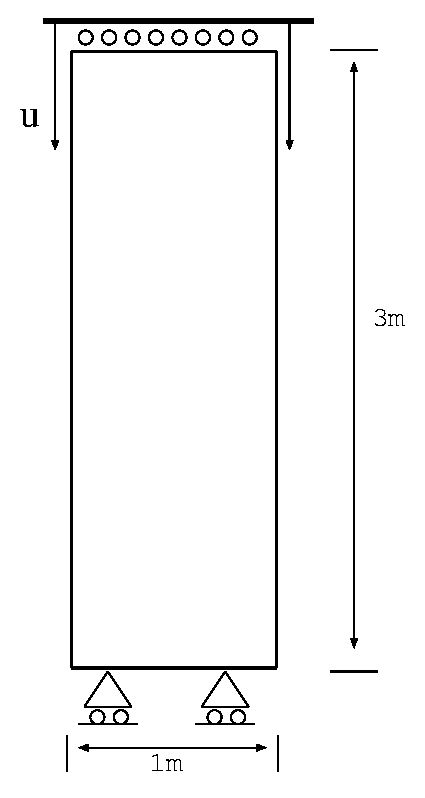
\includegraphics[scale=0.45]{M/biaxial.eps}
\caption{Plane strain biaxial test}
 \label{fig:biaxial}
\end{figure}

\subsubsection*{Boundary conditions}

The bottom of the specimen is placed on horizontal roll supporters.
While the top of it is only allowed to a vertical down movement
$u_z$. Both lateral sides are considered to be traction free.

\subsubsection*{Material properties}

The non-associative flow rule is adopted for the Drucker-Prager model. All material parameters are given in Table (\ref{ex1:tableDP})

\begin{table}[H]
\centering
\begin{tabular}{lll}
\hline \hline
Parameter   &  Unit  & Value\\
\hline
  Young's modulus &  $kPa$ &  $2\times10^4$ \\
\hline\hline
  Poisson ratio & - &  0.4 \\
\hline
  Parameter $\alpha$  & - & 0.233345 (30$^\circ$ friction angle)\\
\hline
  Parameter $\beta$  & - &  0.141421 (16.53$^\circ$ dilatancy angle)\\
\hline
  Initial stress $\sigma_0$ & $kPa$ &  29.69 (20 of initial cohesion)\\
\hline
  Hardening modulus $H$ & $kPa$ &  100\\
\hline
  Localized softening modulus $H_{\delta}$ & $kPa$ & -1000, varying\\
\hline \hline
\end{tabular}
\caption{Material parameters of the plane strain biaxial test}
\label{ex1:tableDP}
\end{table}

\subsubsection*{Results}
Fig. \ref{fig:loc} shows the deformed sample exhibiting localization. Fig. \ref{fig:vreact} depicts the stress
reaction at the top surface due to the displacement load. The results agrees with what given in \cite{Bo00}

\begin{figure}[H]
\begin{center}
\includegraphics[scale=0.35]{M/m_sdc.eps}
\end{center}
\caption{Vertical reaction of the top}.
 \label{fig:loc}
\end{figure}
\begin{figure}[H]
\begin{center}
\includegraphics[scale=0.35]{M/m_sdc_s_u.eps}
\end{center}
\caption{Vertical reaction of the top}.
 \label{fig:vreact}
\end{figure}

\subsubsection*{Benchmark deposit}
\begin{tabular}{|l|l|l|}
  \hline
  Benchmark & Problem type & Path in benchmark deposit \\
  \hline
 \emph{m\_sdc} & M & benchmarks\verb \M\ \\
  \hline
\end{tabular}


%-------------------------------------------------------------------------
\subsection{Plastic plate - Cam-Clay plasticity (2D)}
\label{sec:ccup}

\subsubsection*{Problem definition}

This example is generally applied to verify a critical state plastic
mode, i.e. Cam-Clay model. We consider a quarter of the cylindrical
sample of 5cm in diameter and 10cm in length.

\subsubsection*{Initial and Boundary conditions}

The bottom surface is roller supported.
A vertical down displacement is prescribed to make an axial strain of 50\%. The movement in the radial
direction on the top surface is allowed. The cylindrical  surface is traction free.

\subsubsection*{Material properties}

Table \ref{tab:m_cc_s} shows the material parameters.
 \begin{table}[H]
\begin{tabular}{lrl}
\hline\noalign{\smallskip}
  \hline
 Meaning & Value & Unit \\
  \hline
 Poisson ratio & $0.3$ & ---\\
 Slope of the critical state line & $1.2$ & ---\\
 Virgin compression index & $0.2$ & ---\\
 swelling/recompression index & $0.02$ & ---\\
 Initial preconsolidation pressure & $60.0$ & $--$\\
 Initial void ratio & $1.5$ & $--$\\
 \hline\hline
\end{tabular}
\caption{Solid material properties} %\footnotesize
\label{tab:m_cc_s}
\end{table}

\subsubsection*{Results}

The problem is axisymmetrical. A relationship between von Mises type stress, the second stress invariant, and the axial strain is illustrated in Fig. \ref{fig:m_cc_s_r}. The results agrees with what given in \cite{SheSloYu00}.

\begin{figure}[H]
  \begin{center}
    \includegraphics[scale=0.3]{M/cc_s_s_e.eps}
  \end{center}
  \caption{Axial strain vs von Mises type stress }
  \label{fig:m_cc_s_r}
\end{figure}

\subsubsection*{Benchmark deposit}

\begin{tabular}{|l|l|l|}
  \hline
  Benchmark & Problem type & Path in benchmark deposit \\
  \hline
 \emph{m\_cc\_quad\_s}\&  \emph{m\_cc\_tri\_s}& M & benchmarks\verb \M\ \\
  \hline
\end{tabular}


%-------------------------------------------------------------------------
\subsection{Plastic plate - Rotational hardening plasticity (2D)}

\subsubsection*{Problem definition}

This example is a plane strain compression test on a
material with both isotropic and rotational hardening behaviour.

The geometry of the specimen used is $0.34$~m height and $0.1$~m
width. We denote by $\sigma_x$ the stress acting on the both
lateral sides of the specimen and by $\sigma_y$ the stress applied
to the top side of the specimen.
 The set-up of the problem is shown in Fig.~\ref{fig:ssy}.

\begin{figure}[H]
\center
\includegraphics[scale=0.3]{M/ssy_mesh.eps}
\caption{Plane strain biaxial test: rotational hardening}
 \label{fig:ssy}
\end{figure}

A vertical down displacement load is applied on the top boundary.

\subsubsection*{Material properties}

Assume all initial stresses are zero. The material properties of the rotational hardening model
are defined in Table \ref{Tab_par_oedo}
\begin{table}[!htb]
\centering
\begin{tabular}{lll}
\hline \hline
Parameter   &  Unit  & Value\\
\hline
  Young's modulus &  Pa &  1e+08 \\
\hline
  Poisson ratio & - &  0.3 \\
\hline
  $\alpha_0$       &  -        & 0.0 \\
  $\beta_0$        &  -        & 0.26 \\
  $\delta_0$       &  $m^2/N$  & 3.5e-07\\
  $ \varepsilon_0$ &  $m^2/N$  & 1.0e-7\\
  $\kappa_0$       &  $N/m^2$  & 0.0  \\
  $\gamma_0$       &  -        & 0.0 \\
  $m_0$            &  -        & 0.569 \\
\hline
  $\hat {\alpha}$  &  -        & 0.0 \\
  $\hat {\beta_0}$ &  -        & 0.29\\
  $\hat{\delta_0}$ &  $m^2/N$  & 8.81e-9\\
  $\hat{\varepsilon_0}$&  $m^2/N$  & 1.5e-8 \\
  $\hat{\kappa_0}$ &  $N/m^2$  & 0.0  \\
  $\hat{\gamma_0}$ &  -        & 0.0 \\
  $\hat{m_0}$      &  -        & 1.0 \\
\hline
  $\psi_1$         &   -       & 0.55\\
  $\psi_2$         &  -        & -0.26\\
\hline
  $C_h$            &  -        & 0.81e-3\\
  $C_d$            &  -        & 0.60e-3\\
\hline
  $b_r$            &  -        & 100.0\\
  $m_r$            &  -        & -3.0\\
\hline \hline
\end{tabular}
\caption{\label{Tab_par_oedo}Material parameters of rotational hardening
model }
\end{table}

\subsubsection*{Results}

The output of the results in a
specified point, i.e, a center of a finite element close to the
geometrical center of the domain (Fig.~\ref{fig:ssy}), is used to analyze the model behavior.
Fig. \ref{fig:ssy_u_s} shows the varying of vertical stress along with vertical displacement at the top boundary.

\begin{figure}[!htb]
\center
\includegraphics[scale=0.4]{M/ssy_u_s.eps}
\caption{Vertical stress vs vertical displacement}
 \label{fig:ssy_u_s}
\end{figure}

\subsubsection*{Benchmark deposit}

\begin{tabular}{|l|l|l|}
  \hline
  Benchmark & Problem type & Path in benchmark deposit \\
  \hline
 \emph{m\_ssy\_quad}& M & benchmarks\verb \M\ \\
  \hline
\end{tabular}




%\section{Localization - Fracture Mechanics}
%\subsection{Fractured plate - Drucker-Prager plasticity (2D)}

\section{Creep}

Creep is a time-dependent and/or temperature-dependent deformation
process of a solid body under the influence of a constant load.
%
Creep is a phenomenon of time effect to deformation such that the
tendency of a material to move or to deform is permanent to relieve
stresses. Similar to plastic potential, a creep potential $F_c$ is
introduced to describe the constitutive equations.

Usually, a stationary creep model is sufficient to describe the
creep phenomena in geological media, such as soil and rock. Norton's
model reads that the creep potential $F_c$ can be expressed by a
function of the first stress invariant $\sivi$ as
%
\begin{equation}
F_c = \frac{\alpha}{n+1}\,\sivi^{n+1}
\end{equation}
%
where $\alpha$ and $n$ are material parameters, which have to be
determined by experiments.
%
Assuming the total strain increment $d \Stra$ is admissible to be
decomposed in several portions contributed by different physical
reactions such elasticity, plasticity and creep, it can be written
as
%
\begin{equation}
d \Stra = d \Stra^{e}+d \Stra^{p}+d \Stra^{c}
\end{equation}
%
Similar to the plastic flow rule, we can derive the strain rate
resulting from creep as
%
\begin{equation}
d \Stra^{c}
=
\frac{ \partial F_c}{\partial \Stress}
=
\left(\frac{3}{2}\right)^{(n+1)/2}
\alpha\left\Vert {\devS}
\right\Vert^{n-1}\devS
\label{eq:crpflow}
\end{equation}

Applying explicit Euler's method to equation (\ref{eq:crpflow}), the
increment of the strain by creep is obtained from
%
\begin{equation}
\Delta \Stra^{c}  =
\left(\frac{3}{2}\right)^{\frac{n+1}{2}}\alpha\norm{\devS^k}^{n-1}\devS^k
\Delta t \label{eq:dstrain_crp}
\end{equation}
%
where $\devS^k$ is the deviatoric stress of the previous time step
$k$ and $ \Delta t$ is the time step size.
%
Using the generalized Hook's law, the stress change deduced by the
creep stain increment is
%
\begin{equation}
\Delta \Stress^{c}  =  \mathbf D^{e} \Delta \Stra^{c}
\label{eq:dstress_crp}
\end{equation}
%
with $\mathbf D^{e}$ the elastic material tensor.


\subsection{Creep of a cylindrical sample}

\subsubsection*{Problem definition}

In this example, creep is considered in a thick cylinder subjected a
constant normal pressure at the inner face.
%
The boundary conditions are as follows: $p$ =2.515 MPa at the inner
surface and zero normal stress at the outer surface, no
displacements in axial direction. The inner radius of the
cylindrical sample is 4 mm, the outer radius is 6.4 mm and the
height is 1 mm. Quadrilateral elements are adopted for meshing (Fig.
\ref{fig:meshcrp}).
%
\begin{figure}[!htb]
\centering
\includegraphics[scale=0.3]{M/mesh_crp}
\caption{Mesh for thick cylinder undergos creep deformation}
\label{fig:meshcrp}
\end{figure}

We assume that the initial stress is homogeneously distributed in
the domain as $\sigma_{r}^0=\sigma_{\theta}^0=\sigma_{z}^0=-50$ Pa.
The parameters of the Norton creep model are given in Tab.
\ref{tab:creep_norton}.

\begin{table}[H]
\center
\begin{tabular}{llrl}
\hline\noalign{\smallskip}
\hline
Symbol & Meaning & Value & Unit \\
\hline
$\alpha$ & Norton model parameter 1 & $6.415\times 10^{-10}$ & -- \\
$n$      & Norton model parameter 2 & $4$ & -- \\
$\nu$    & Poisson ratio & $0.48$ & -- \\
$E$      & Young's modulus & $1.378\times10^5$ & MPa \\
\hline\hline
\end{tabular}
\caption{Material parameters of the Norton creep model} %\footnotesize
\label{tab:creep_norton}
\end{table}


\subsubsection*{Results}

Figs. \ref{fig:ex2_q} and \ref{fig:ex2_ur} give the distribution of
the first stress invariant and radial displacement along radial
direction and the comparison with pure elastic solution. They
demonstrated that $\mathbf s$ at inner surface decreases about 26\%
after steady state of creep reached. While radial displacements
increase about 200\%.
%
The results can be compared with Balley's analytical solution, which
reads for rate of radial displacement as
%
\[
  \dot u_{r} =\alpha \dfrac{3^{\frac{n+1}{2}}}{2n^n}\dfrac{r_{a}^2\;r_{b}^2\;p^n}{(r_{b}^{2/n}-r_{a}^{2/n})r}
%% \label{eq:balleyu}
\]
and for the steady state of first stress invariant
\[
  \sigma_v =\dfrac{2\sqrt 3}{2n} \dfrac{p\;\left(r_b/r\right)^{\frac{2}{n}}}{(r_{b}/r_a)^{2/n}-1}
%% \label{eq:balleys}
\]

\subsubsection*{Benchmark deposit}
\begin{tabular}{|l|l|l|}
  \hline
  Benchmark & Problem type & Path in benchmark deposit \\
  \hline
 \emph{m\_crp\_tri}& M & benchmarks\verb \M\ \\
  \hline
\end{tabular}

\begin{figure}[H]
\centering
\includegraphics[scale=0.4]{M/crp/ex2_q}
\vspace{-3mm}
\caption{First stress invariant profiles during creep at different times, $t$ = 5,25,50 sec,
and comparison to elastic solution}
\label{fig:ex2_q}
\end{figure}

\begin{figure}[H]
\centering
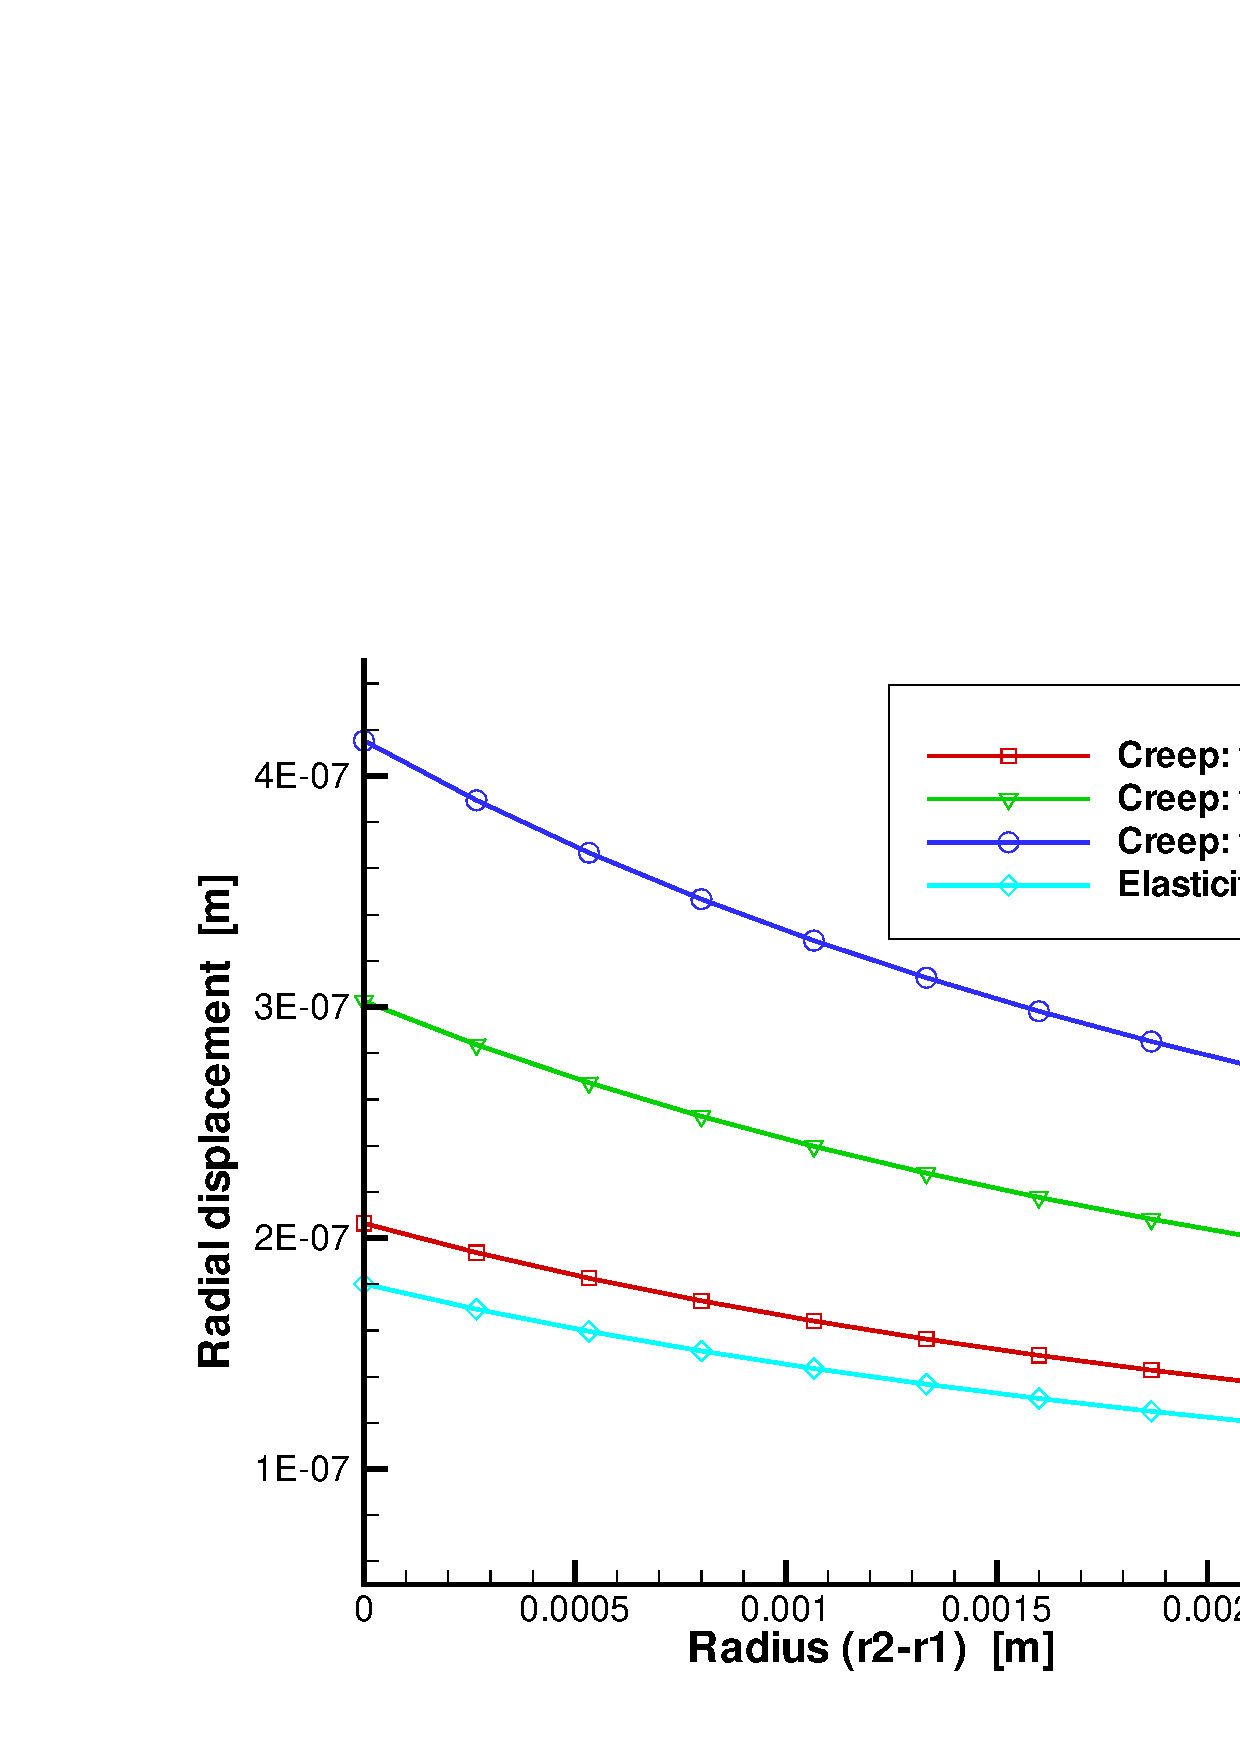
\includegraphics[scale=0.4]{M/crp/ex2_ur}
\vspace{-3mm}
\caption{Radial displacement profiles during creep at different times, $t$ = 5,25,50 sec,
and comparison to elastic solution}
\label{fig:ex2_ur}
\end{figure}


\newpage
%-------------------------------------------------------------------------
\subsection{Creep in salt rock}

Several models exists for the evaluation of the effect of stationary
creep in rock salt, i.e the strain variation with time is
calculated. One of those models is the BGRa-model
(\ref{eqn:BGRa_model}), which is valid for loads between 5 and 25
MPa in a temperature range of 22-200$^o$C (Hunsche and Schulze,
1994).
%
\begin{equation}
\dot\Stra^{c}
=
A e^{-\frac{Q}{R T}}
\left( \frac{\sigma}{\sigma^*} \right)^n
\label{eqn:BGRa_model}
\end{equation}
%
Table \ref{tab:creep_salt} depicts the symbols of equation
(\ref{eqn:BGRa_model}), their meaning and parameter values.
%
\begin{table}[H]
\center
\begin{tabular}{llrl}
\hline\noalign{\smallskip}
\hline
Symbol & Meaning & Value & Unit \\
\hline
$\dot\Stra$ & Strain rate & & 1/d \\
$\sigma$ & Effective stress & $$ & MPa \\
\hline
$A$ & Material constant & $0.18$ & 1/d \\
$Q$ & Activation energy & $54$ & kJ/mol \\
$R$ & Gas constant & $8.31447215$ & J/(K mol) \\
$n$ & Material constant & $5$ & -- \\
$\sigma^*$ & Reference effective stress & $1$ & MPa \\
\hline\hline
\end{tabular}
\caption{Creep model, symbols and material values} %\footnotesize
\label{tab:creep_salt}
\end{table}

\subsubsection*{Example 1: Temperature dropping (relaxation)}
\label{sec:creep_salt_example_1}

\paragraph*{Problem definition}
In a sample of rock salt a stress relaxation is caused by a
temperature decrease of 30 K. The aim of the example is to calculate
the resulting strain variation with time within the solid body by
the use of the stationary creep model BGRa (\ref{eqn:BGRa_model}).
The results of the simulation using an axial symmetric calculation
model and a 3D model are compared afterwards.

Assumptions
\begin{tabular}{|ll|}
\hline\noalign{\smallskip}
Heat  & Constant temperature in the whole body at the \\
      & beginning (330 K), temperature decrease of 30 K \\
Solid & Homogenous, finite dimensions, no deformation at the \\
      & boundaries in z-direction at the bottom and the top \\
\hline
\end{tabular}

\begin{figure}[H]
\centering
\includegraphics[scale=0.5]{M/creep_salt_1}
\caption{Core sample model}
\label{fig:creep_salt_1}
\end{figure}

For the 2D numerical simulation a cylindrical core sample as shown
in Fig. \ref{fig:creep_salt_1} is selected. The 2D numerical model
is an axial symmetric one in the x-z-plane (see Fig.
\ref{fig:creep_salt_2}). The dimensions of this 2D model are: 0.05 m
radius (x-direction) and 0.2 m of height. A relatively coarse mesh
consisting of 228 triangular elements and 139 nodes is used.
Vertical deformations at the top and the bottom are suppressed (no
displacement boundary conditions). The initial temperature in the
whole area is 330 K. At the top and the bottom of the model thermal
boundary conditions are set with a temperature of 300 K. Thereby the
stress relaxation during the cooling down is simulated. The used
parameters of the solid represent the material behavior of rock salt
are given in Tab. \ref{tab:creep_salt}. The calculation is divided
in 360 time steps with a constant time step length of 1 day.

\begin{figure}[H]
\centering
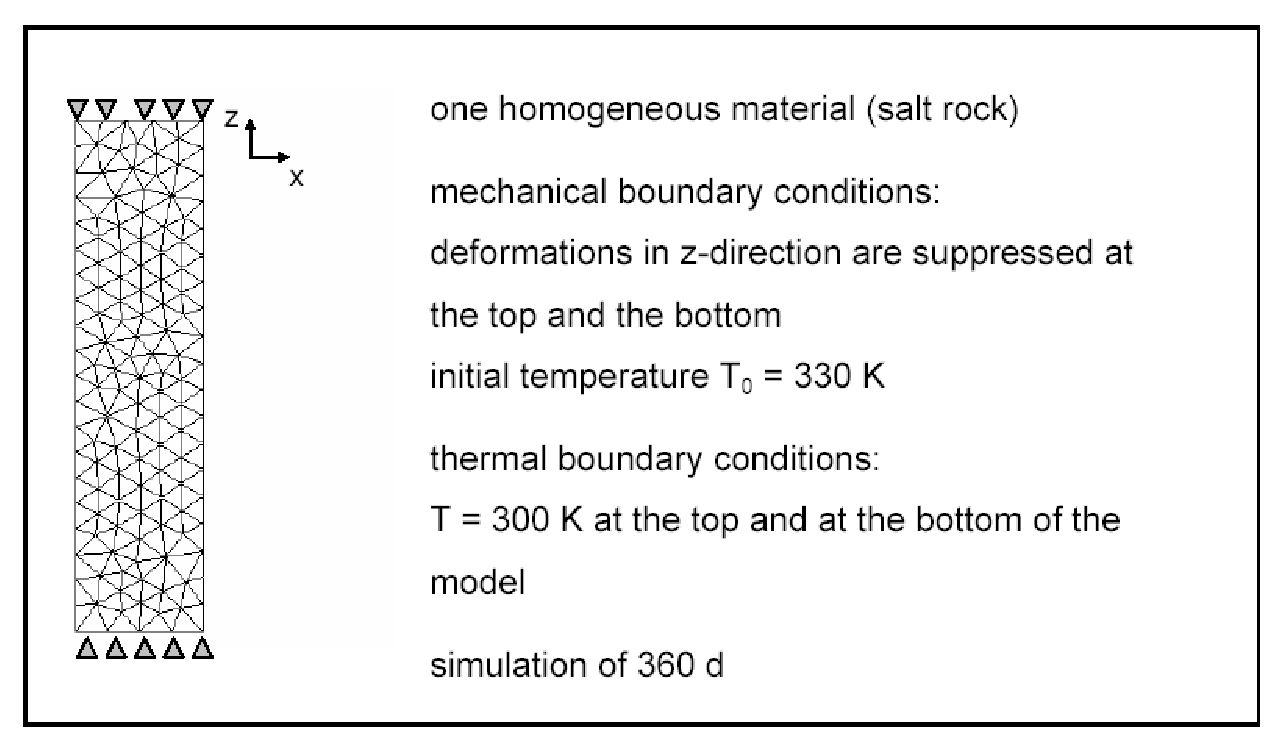
\includegraphics[scale=0.5]{M/creep_salt_2}
\caption{Numerical axisymmetrical model} \label{fig:creep_salt_2}
\end{figure}

Table \ref{tab:creep_salt_heat} depicts the values of material
properties for the thermo-mechanical creep model.
%
\begin{table}[H]
\center
\begin{tabular}{llrl}
\hline\noalign{\smallskip}
\hline
Symbol & Meaning & Value & Unit \\
\hline
$T_0$    & Initial temperature (before cooling down) & $330$ & K \\
$T$      & Temperature after cooling down & $300$ & K \\
$E$      & Young's modulus & $25$ & GPa \\
$\nu$    & Poisson ratio & $0.27$ & -- \\
$\alpha$ & Thermal expansion coefficient & $4\times 10^{-5}$ & 1/K \\
$c$      & Thermal capacity & $1$ & J/(kg K) \\
$\lambda$ & Thermal conductivity & $100$ & W/(m K) \\
\hline\hline
\end{tabular}
\caption{Material parameters of the thermo-mechanical creep model} %\footnotesize
\label{tab:creep_salt_heat}
\end{table}

\paragraph*{Analytical solution}
%
In order to evaluate the numerical results of the relaxation
problem, the analytical solution of equation
(\ref{eqn:BGRa_model_2}) (Eickemeier 2007, personal communication)
for the difference of effective stresses within one time step can be
applied.
%
\begin{equation}
\Delta\sigma_{i+1}
=
\frac
{(\dot\Stra^{c}_1 - A (\sigma/\sigma^*)^n) E_q \Delta t}
{1 - E_q / \sigma^* A^* \Delta t \xi n (\sigma/\sigma^*)^{n-1}}
\label{eqn:BGRa_model_2}
\end{equation}
%
and
%
\begin{equation}
A^*
=
A e^{-Q/RT}
\label{eqn:BGRa_model_3}
\end{equation}
%
where the initial strain rate $\dot\Stra^{c}_1$ in this case is
zero, $E_q$ in general is the weighted Young's modulus of the steel
plates and the salt rock sample (in this case we consider only salt
rock), $\xi$ = 0.5.

For the analytical solution of the equation (\ref{eqn:BGRa_model_2})
the vertical stress before the last time step is considered. Time
step increment is $\Delta t$ = 1 d. The calculation is done for node
705 of the 3D model (Fig. \ref{fig:creep_salt_3}), which is located
at point (x,y,z)=(0.05,0,0.12). The calculated stress difference
$\sigma_{i+1}$ has to be identical to the numerical result.

\begin{figure}[H]
\centering
\includegraphics[scale=0.28]{M/creep_salt_3}
\caption{Comparison of numerical results (GeoSys/RockFlow vs ANSALT) for vertical stresses}
\label{fig:creep_salt_3}
\end{figure}

\paragraph*{Results}
%
The comparison of the stress increment $\sigma_{i+1}$ which was
obtained by the use of equation (\ref{eqn:BGRa_model_2}) is
identical to the value (of vertical stresses) at node 705 (at the
same location as node 76, see Fig. \ref{fig:creep_salt_3}) of the 3D
numerical calculation. Both stress increments $\sigma_{i+1}$
obtained by GS/RF and ANSALT are equal to $3.05\times 10^{-3}$ MPa.
Additionally, the numerical results for vertical stresses of the 2D
simulation at node 76 are compared to the results that were obtained
by simulating the creep process by the FE programme ANSALT (Nipp
1988) and also to the results of the 3D simulation with GS/RF at
node 705. The comparison of the results of GS/RF in 2D and 3D with
the ANSALT findings are depicted in Fig. \ref{fig:creep_salt_3}.

The input data and boundary conditions for each calculation model
are identical. Also the results show a good accordance. That means,
the creep simulation (2D and 3D) of GS/RF by using the implemented
BGRa model provides correct results.

\subsubsection*{Benchmark deposit}

\begin{tabular}{|l|l|l|l|l|l|}
\hline
PCS type & MSH type       & Files   & Version    & Date    & Author\\
\hline
TM       & axial-symmetry & BGRa    & 4.4.10(WW) & 13.03.07 & BGR \\
\hline
TM       & axial-symmetry & creep3d & 4.4.10(WW) & 13.03.07 & BGR \\
\hline
\end{tabular}

%-------------------------------------------------------------------------
\subsubsection*{Example 2: Creep under constant load}

\paragraph*{Problem definition}
%
In the same example that is described in section
\ref{sec:creep_salt_example_1} the creep process is now assumed to
be caused by a constant load at the bottom of the solid and a
constantly high temperature at the same time. The aim of this
example is to calculate the resulting strain variation with time by
using the stationary creep model BGRa (\ref{eqn:BGRa_model}).

We specify the initial and boundary conditions for the 2D numerical
model. For the simulation with GS/RF almost the same calculation
models (2D and 3D) as in the precedent creep example were selected.
Only the height of the solid is 0.25 m instead of 0.2 m. The initial
temperature in the whole area is 373.15 K. There is a constant load
of 5 MPa at the bottom of the model as boundary condition. The
calculation is divided in 100 time steps with a constant time step
length of 1 day.

\paragraph*{Analytical solution}
%
In order to find out, whether the numerical solutions of
GeoSys/RockFlow accord to the results of the BGRa model
(\ref{eqn:BGRa_model}), the input parameter $A$ is compared to the
$A$, which results from the simulation run. For this calculation
equation (\ref{eqn:BGRa_model}) is converted to the following
expression.
%
\begin{equation}
A
=
\frac
{\dot\Stra^{c}}
{e^{-Q/RT} \sigma_{\mbox{\footnotesize eff}}}
\label{eqn:BGRa_model_4}
\end{equation}
%
with
%
\begin{eqnarray}
\sigma_{\mbox{\footnotesize eff}}
&=&
\frac{1}{\sqrt{2}}
\sqrt{(\sigma_1-\sigma_2)^2 + (\sigma_2-\sigma_3)^2 + (\sigma_3-\sigma_1)^2}
\nonumber
\\
\dot\Stra
&=&
\frac
{\Stra_{\mbox{\footnotesize eff}}(t+\Delta t) - \Stra_{\mbox{\footnotesize eff}(t)}}
{\Delta t}
\\
\Stra_{\mbox{\footnotesize eff}}
&=&
\frac{\sqrt{2}}{3}
\sqrt{(\Stra_1-\Stra_2)^2 + (\Stra_2-\Stra_3)^2 + (\Stra_3-\Stra_1)^2}
\nonumber
\label{eqn:BGRa_model_5}
\end{eqnarray}

For these calculation steps the stresses of the regarded time period
have to be constant. Equations (\ref{eqn:BGRa_model_5}) are solved
for node 25 (see Fig. \ref{fig:creep_salt_4}) of the 2D numerical
model. The last time step at $t$ = 100 days of the simulation run
was considered.
%
\begin{figure}[H]
\centering
\includegraphics[scale=0.26]{M/creep_salt_4}
\caption{Comparison of 2D and 3D numerical results for strains (x- and z-directions)}
\label{fig:creep_salt_4}
\end{figure}
%
\begin{figure}[H]
\centering
\includegraphics[scale=0.37]{M/creep_salt_5}
\caption{Comparison of 2D and 3D numerical results for strains (y-direction)}
\label{fig:creep_salt_5}
\end{figure}

\paragraph*{Results}
%
The effective stress $\sigma_{\mbox{\footnotesize eff}}$ at node 25
and for the given time span is 5.03 MPa, which was calculated by the
use of equation (\ref{eqn:BGRa_model_5}). The strain of time step 1
is $\Stra_{\mbox{\footnotesize eff}}(t_1)$ = $1.72\times 10^{-3}$
and of time step 2: $\Stra_{\mbox{\footnotesize eff}}(t_2)$ =
$1.73\times 10^{-3}$ , calculated by equation
(\ref{eqn:BGRa_model_5}), is equal to $1.6 \times 10^{-5} d^{-1}$.
After equation (\ref{eqn:BGRa_model_4}) the calculated parameter $A$
is equal to 0.19, which corresponds approximately to the input $A$
of 0.18. Therefore, it can be summarized that the BGRa creep model
is implemented in GeoSys/RockFlow properly. The comparison between
the 2D (node 25) and 3D results (node 705) are depicted in Fig.
\ref{fig:creep_salt_4} and Fig. \ref{fig:creep_salt_5}. The 2D and
3D results are identical to each other.

\subsubsection*{Benchmark deposit}

\begin{tabular}{|l|l|l|l|l|l|}
\hline
PCS type & MSH type       & Files     & Version    & Date    & Author\\
\hline
M       & axial-symmetry & uc\_creep01 & 4.4.10(WW) & 13.03.07 & BGR \\
\hline
M       & axial-symmetry & uc\_creep3d & 4.4.10(WW) & 13.03.07 & BGR \\
\hline
\end{tabular}



\clearpage

\subsection{Lubby2: Transient and stationary creep model}
\label{subsec:lubby2}

Viscoplastic creep is mainly caused by diffusion and dislocations at the microscale, and results in hardening as well as recovery aspects. Hou and Lux propose an evolutional equation for the (viscoplastic) creep strain rate considering stationary as well as transient creep, damage impact, hardening and recovery (cf. \cite{Hou:1997,Hou:2002,HL:1998}). Neglecting damage effects, this approach is known as Lubby2 model.
\begin{equation}
\mio{\varepsilon}{\mathrm{c}}{\dot}\,=\,
\frac{3}{2}\,
\left[
\frac{1}{\eta_k}
\left(
1\,-\,
\frac{\varepsilon^{\mathrm{tr}}}{\mathrm{max}\,\varepsilon^{\mathrm{tr}}}
\right)
\,+\,\frac{1}{\eta_m}
\right]
\,\mio{s}{}{}
\label{lubby2_ec}
\end{equation}

Here $\mio{s}{}{}$ denotes the deviatoric stress tensor
\begin{equation}
\mio{s}{}{}\,=\,\mio{\sigma}{}{}\,-\,\frac{1}{3}(\mathrm{tr}\,\mio{\sigma}{}{})\,\mio{I}{}{}
\end{equation}
and $\varepsilon^{\mathrm{tr}}$ the equivalent transient creep strain
\begin{equation}
\varepsilon^{\mathrm{tr}}\,=\,
\sqrt{\frac{2}{3}\,\mio{\varepsilon}{\mathrm{tr}}{}\ccdot\mio{\varepsilon}{\mathrm{tr}}{}}
\end{equation}
with $\mio{\varepsilon}{\mathrm{tr}}{}=\mio{\varepsilon}{\mathrm{c}}{}-\mio{\varepsilon}{\mathrm{st}}{}$ ($\mio{\varepsilon}{\mathrm{st}}{}$ -- stationary creep fraction). In addition to the equivalent transient creep strain the generalized representation of the von~Mises equivalent deviatoric stress $s_{\mathrm{v}}$ is defined.
\begin{equation}
s_{\mathrm{v}}\,=\,\sqrt{\frac{3}{2}\,\mio{s}{}{}\ccdot\mio{s}{}{}}
\end{equation}

Furthermore, the following material functions are suggested, considering only hardening, and neglecting recovery effects:
\begin{eqnarray}
\mathrm{max}\,\varepsilon^{\mathrm{tr}} & \!\!\!\!= &
\!\!\!\!\frac{s_{\mathrm{v}}}{G_k}
\\[2.0ex]
G_k & \!\!\!\!= &
\!\!\!\!{\bar G}^{\ast}_k\,\mathrm{exp}
\left(
k_1\,s_{\mathrm{v}}
\right)\;\,\qquad\qquad\mbox{(Kelvin shear modulus)}
\label{lubby2_f2}
\\[2.0ex]
\eta_k & \!\!\!\!= & \!\!\!\!{\bar\eta}^{\ast}_k\,\mathrm{exp}
\left(
k_2\,s_{\mathrm{v}}
\right)\;\;\,\qquad\qquad\mbox{(Kelvin viscosity modulus)}
\label{lubby2_f3}
\\[2.0ex]
\eta_m & \!\!\!\!= & \!\!\!\!{\bar\eta}^{\ast}_m\,\mathrm{exp}
\left(
m\,s_{\mathrm{v}}
\right)\,\mathrm{exp}(lT)\quad\mbox{(Maxwell viscosity modulus)}
\label{lubby2_f4}
\end{eqnarray}

As $\;T$ denotes the absolute temperature, the following material
parameters are necessary to model various constitutive effects:
\begin{list}{$\bullet$}{\topsep0mm \partopsep0mm \leftmargin6mm
   \parsep0ex \itemsep0.75ex}
\item ${\bar G}^{\ast}_k\,,\;k_1$ \hspace*{3.0ex} hardening,
%\item ${\bar G}^{\ast}_{kE}\,,\;k_{1E}$ \hspace*{0.4ex} recovery,
\item ${\bar\eta}^{\ast}_k\,,\;k_2$ \hspace*{4.0ex} transient creep, and
\item ${\bar\eta}^{\ast}_m\,,\;m\,,\;l$ \hspace*{1.0ex} stationary creep.
\end{list}

\clearpage

\subsubsection*{Problem definition}

Triaxial long-term compression under axisymmetric conditions is carried out to verify the Lubby2 creep model, and to study transient as well as stationary creep behavior assuming isothermal conditions and neglecting damage processes. As described in Sec.~\ref{subsec:lubby1}, for the calculation, the cross-section of a cylindrical sample with a radius of 30~mm and a height of 120~mm is studied. The loading in principal axes includes a radial pressure as well as an axial pressure, and is realized in two steps. It is resulting in a homogeneous stress-strain state. Details of the model (geometry, mesh, boundary conditions) according to K.-H. Lux and F. Werunsky (unpublished report, 2008) are presented in Fig.~\ref{triax_model_lubby2}.

\begin{figure}[!htb]
\begin{center}
\includegraphics[width=0.2\textwidth]{M/figure/svv_model.eps}
\hspace*{10.0ex}
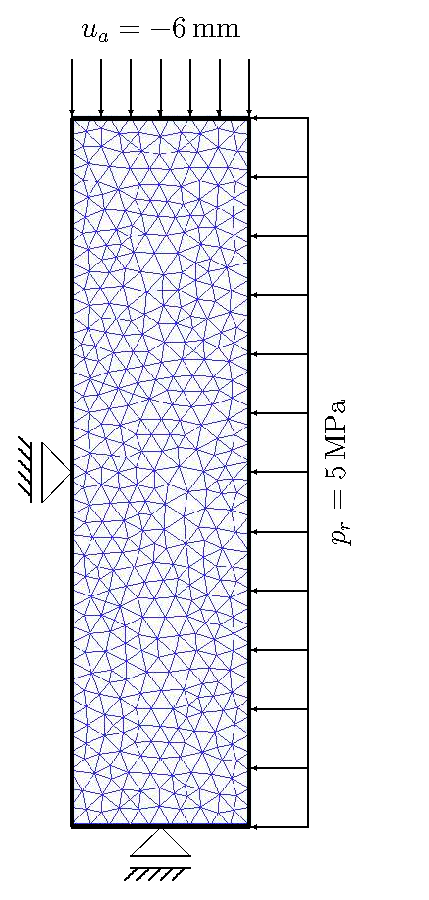
\includegraphics[width=0.25\textwidth]{M/figure/svv_mesh.eps}
\end{center}
\caption{Triaxial compression of a cylindrical sample. Axisymmetric model. Left: Geometry. Right: Finite element grid and boundary conditions.} 
\label{triax_model_lubby2}
\end{figure}

\subsubsection*{Initial and boundary conditions}

Initial conditions do not have to be given for the problem under consideration. As the bottom edge is fixed in vertical direction, the left-hand edge is fixed in horizontal direction for symmetry reasons (axis of rotation). On the right-hand edge initially a radial casing pressure of 5~MPa is applied within 60~seconds with a constant stress rate. While keeping constant this radial pressure, a subsequent stress-driven axial compressive loading is applied within the following 1\,440~seconds with a constant stress rate. The maximum axial pressure is 18~MPa. In the following, both the radial and the axial pressures are kept constant for 20~days (for the loading history cf. Fig.~\ref{triax_loadhist_lubby2}).

\clearpage

\begin{figure}[!htb]
\begin{center}
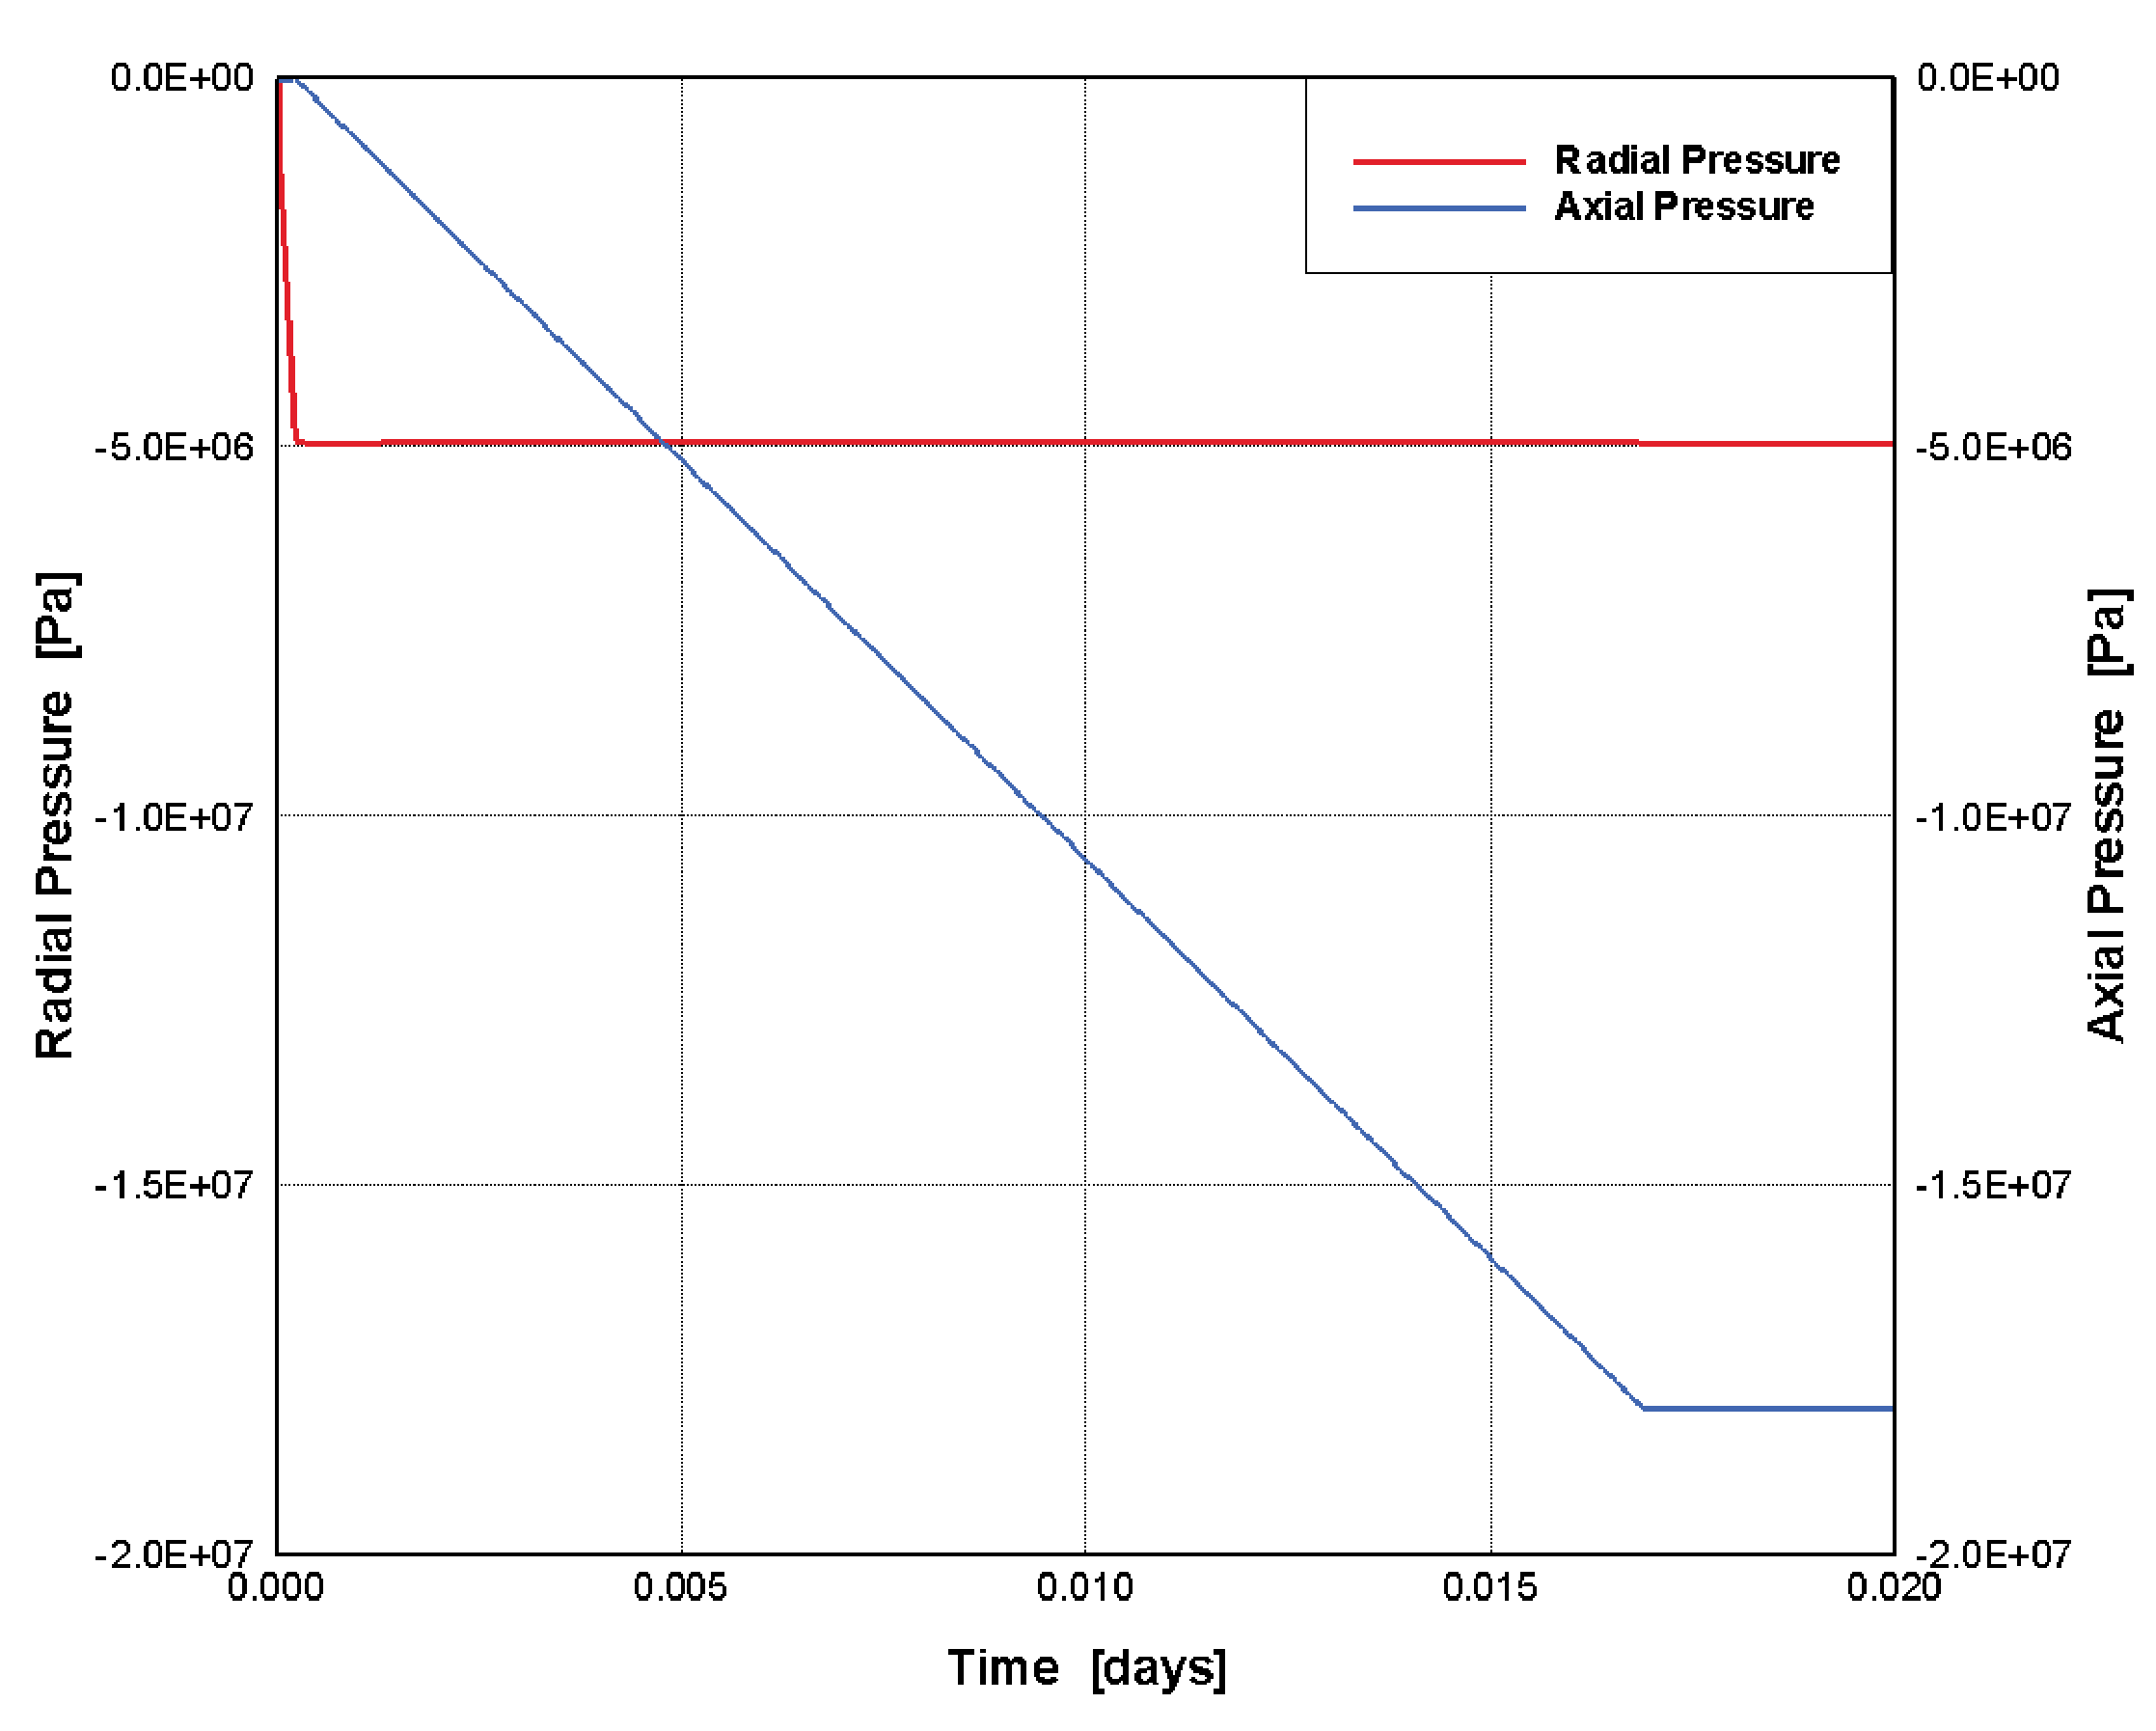
\includegraphics[width=0.6\textwidth]{M/figure/creep/svvcreep_e_HL_loadhistory.eps}
\end{center}
\caption{Triaxial compression of a cylindrical sample. Loading history for long-term creep experiments. Radial casing pressure (stress rate $\dot{p}{}_r=0.083$\,MPa$\cdot$s$^{-1}$) with subsequent axial pressure (stress rate $\dot{p}{}_a=0.0125$\,MPa$\cdot$s$^{-1}$). Each pressure loading with subsequent constant values over 20 days.} 
\label{triax_loadhist_lubby2}
\end{figure}

\subsubsection*{Material properties}

The modified Lubby1 model was considered to generate the fourth-order elastic material matrix for the creep model under consideration. Within this context, the material parameters referring to the modified Lubby1 relation~(\ref{lubby1_ev}) are given in Tab.~\ref{matpar_lubby2_1}. The material parameters for the creep fraction (Lubby2 (\ref{lubby2_ec})) are given in Tab.~\ref{matpar_lubby2_2}. Within this context, the initial Young's modulus, the Poisson's ratio and all the creep parameters are close to values known for rock salt according to K.-H. Lux, M. Rutenberg and F. Werunsky (unpublished report, 2008). 
 
\begin{table}[!htb]
\centering
\begin{tabular}{lll}
\hline\hline\noalign{\smallskip}
Property & Value & Unit \\
\noalign{\smallskip}\hline\noalign{\smallskip}
Poisson's ratio $\nu$             & 0.335   & --  \\
initial Young's modulus $E_0$     & 21\,400 & MPa \\
factor $a$ in (\ref{lubby1_ev})   & 27\,500 & --  \\
exponent $n$ in (\ref{lubby1_ev}) & 1.0     & --  \\
\noalign{\smallskip}\hline\hline
\end{tabular}
\caption{Material parameters for the elastic fraction of the material model (cf.~Sec.~\ref{subsec:lubby1})}
\label{matpar_lubby2_1}
\end{table}
 
\begin{table}[!htb]
\centering
\begin{tabular}{lll}
\hline\hline\noalign{\smallskip}
Property & Value & Unit \\
\noalign{\smallskip}\hline\noalign{\smallskip}
Maxwell viscosity ${\bar\eta}^{\ast}_m$ in (\ref{lubby2_f4})  & $1.09\cdot 10^7$ & MPa$\cdot$day \\
factor $m$ in (\ref{lubby2_f4})                               & $-0.219$         & MPa$^{-1}$    \\
factor $l$ in (\ref{lubby2_f4})                               & $0.0$            & K$^{-1}$      \\
Kelvin viscosity ${\bar\eta}^{\ast}_k$ in (\ref{lubby2_f3})   & $1.45\cdot 10^5$ & MPa$\cdot$day \\
factor $k_1$ in (\ref{lubby2_f2})                             & $-0.146$         & MPa$^{-1}$    \\
factor $k_2$ in (\ref{lubby2_f3})                             & $-0.121$         & MPa$^{-1}$    \\
Kelvin shear modulus ${\bar G}^{\ast}_k$ in (\ref{lubby2_f2}) & $7.0\cdot 10^4$  & MPa           \\
\noalign{\smallskip}\hline\hline
\end{tabular}
\caption{Material parameters for the creep fraction of the material model}
\label{matpar_lubby2_2}
\end{table}


\subsubsection*{Results}

The representation of the axial stress vs. the axial strain in Fig.~\ref{triax_res_lubby2} shows the complex creep behavior of the sample under consideration.

\begin{figure}[!htb]
\begin{center}
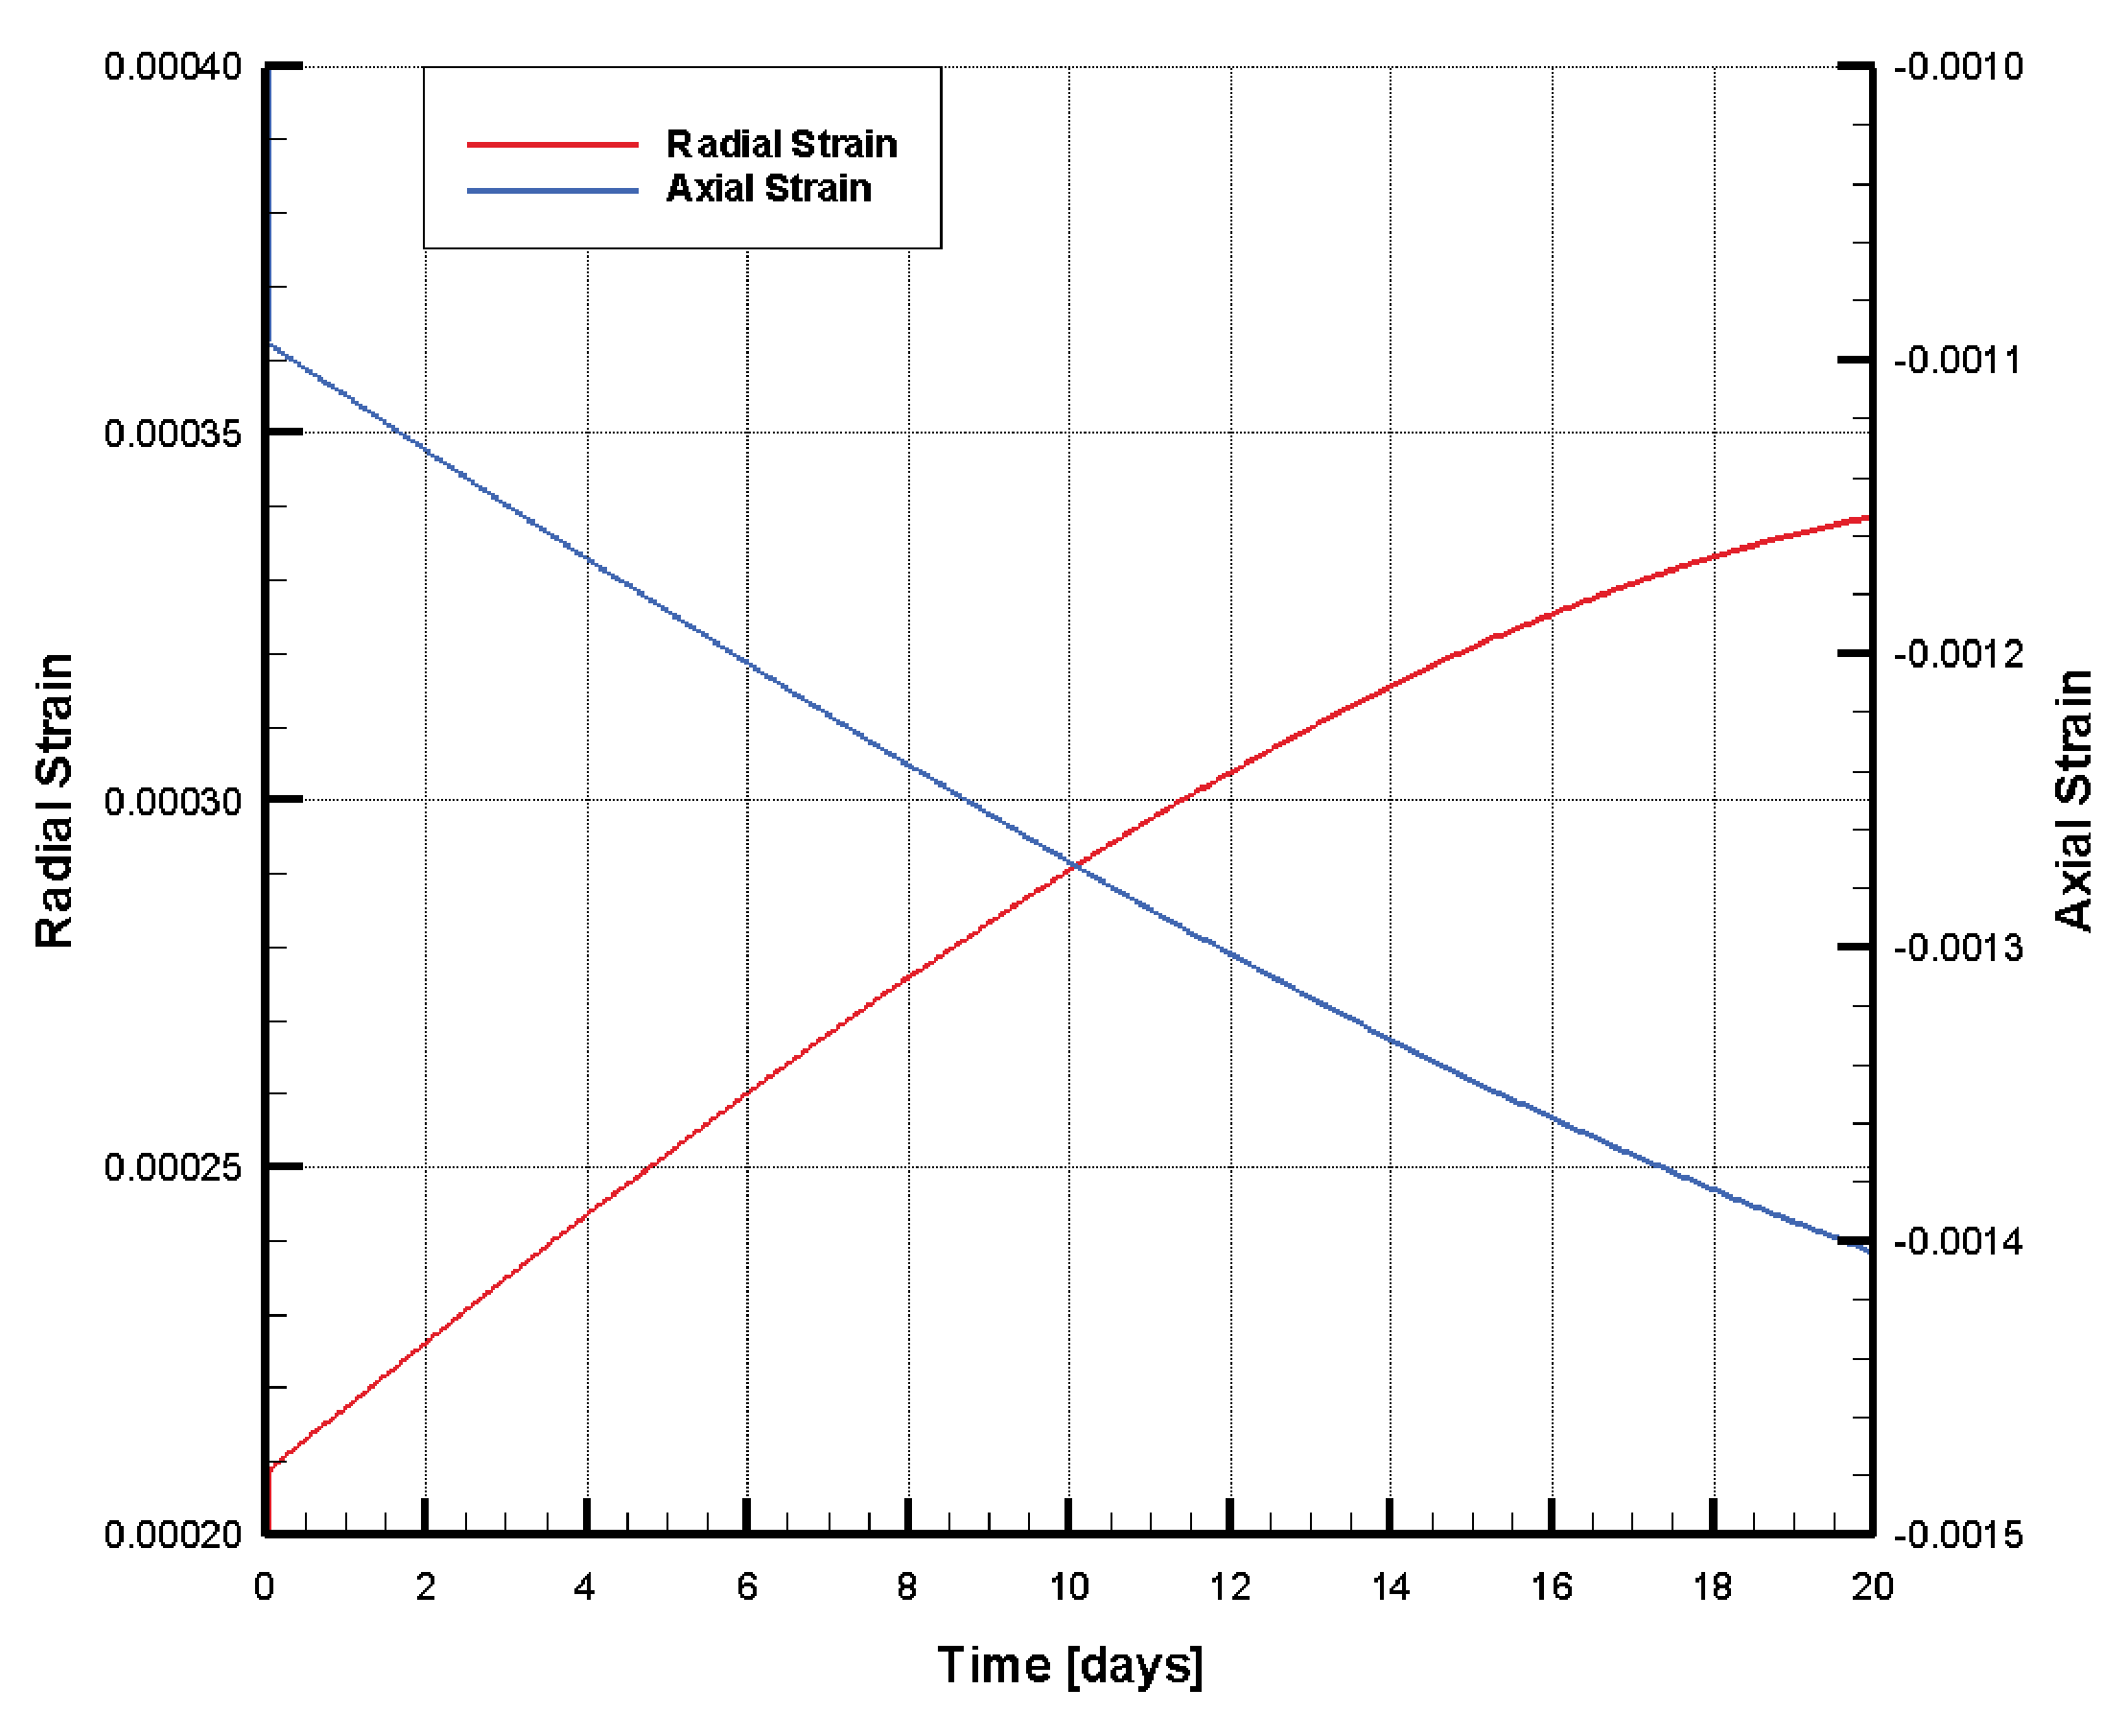
\includegraphics[width=0.6\textwidth]{M/figure/creep/svvcreep_e_HL_strain.eps}
\end{center}
\caption{Triaxial compression of a cylindrical sample. Numerical simulation of the transient and stationary creep behavior using the Lubby2 model~(\ref{lubby2_ec}).} 
\label{triax_res_lubby2}
\end{figure}

\subsubsection*{Benchmark deposit}

\begin{tabular}{|l|l|l|}
  \hline
  Benchmark & Problem type & Path in benchmark deposit \\
  \hline
 \emph{m\_triax\_lubby2} & M & benchmarks\verb \M\creep \\
  \hline
\end{tabular}

